\documentclass{article} %[12pt]{amsart}

\usepackage{arxiv}
\usepackage{geometry} % see geometry.pdf on how to lay out the page. There's lots.
\usepackage{booktabs}
\usepackage{topcapt}
\usepackage{natbib}
\usepackage{array}
\usepackage{url}
\usepackage{hyperref}
\usepackage{graphicx}
\usepackage{todonotes}
\usepackage{listings} % make code listings -MP
\usepackage{minted}   % pretty print code -MP
\usepackage{tablefootnote}

% \geometry{landscape} % rotated page geometry

% See the ``Article customise'' template for come common customisations

\title{Numerical modeling of Earth's dynamic surface: a community approach}



%%%%%%%%%%%%%%%  Author list  %%%%%%%%%%%%%%%
\usepackage{authblk}
\renewcommand*{\Authfont}{\bfseries}
\author[1,2\thanks{Corresponding author; email: \texttt{gtucker@colorado.edu}, twitter: \texttt{@geomorphtucker}}]{Gregory E.\ Tucker}
\author[3]{Eric W.H.\ Hutton}
\author[3]{Mark D.\ Piper}
\author[3]{Benjamin Campforts}
\author[3]{Tian Gan}
\author[1,2,4]{Katherine R.\ Barnhart}
\author[3]{Albert Kettner}
\author[2,3]{Irina Overeem}
\author[3]{Scott D.\ Peckham}
\author[3]{Lynn McCready}
\author[3]{Jaia Syvitski}
\affil[1]{Cooperative Institute for Research in Environmental Sciences (CIRES), University of Colorado Boulder}
\affil[2]{Department of Geological Sciences, University of Colorado Boulder}
\affil[3]{Institute for Arctic and Alpine Research (INSTAAR), University of Colorado Boulder}
\affil[4]{Current address: Landslide Hazards Group, US Geological Survey}

\date{Preprint submitted to EarthArXiv, February 2021 (not peer reviewed)} % delete this line to display the current date

% Uncomment to override  the `A preprint' in the header
\renewcommand{\headeright}{Technical Report / Preprint}
\renewcommand{\undertitle}{Community Surface Dynamics Modeling System (CSDMS) Technical Report \& Preprint}
\renewcommand{\shorttitle}{CSDMS}


%%% BEGIN DOCUMENT
\begin{document}

\maketitle

%[COULD USE A BETTER TITLE..., ]
%[Alternative title: IN FLUX: modeling the ever-evolving Earth Surface needs a community approach   ]
%[Alternative title 1: CSDMS: a community effort to numerically model the dynamics of the Earth’s surface.]
%[NOTE: LET'S CHALLENGE OURSELVES TO USE ACTIVE VOICE. SQUASH `TO BE' EVERYWHERE WE CAN!]

%[ALSO: NOTHING WRONG WITH BRINGING A SENSE OF HUMOR TO SCIENCE WRITING]




\section*{Abstract}

Computational modelling occupies a unique niche in Earth environmental sciences. Models serve not just as scientific technology and infrastructure, but also as digital containers of the scientific community's understanding of the natural world. As this understanding improves, so too must the associated software. This dual nature---models as both infrastructure and hypotheses---means that modelling software must be designed to evolve continually as geoscientific knowledge itself evolves. Here we describe design principles, protocols, and tools developed by the Community Surface Dynamics Modeling System (CSDMS) to promote a flexible, interoperable, and ever-improving research software ecosystem. These include a community repository for model sharing and metadata, interface and ontology standards for model interoperability, language bridging tools, a modular programming library for model construction, modular software components for data access, and a Python-based execution and model-coupling framework. Methods of community support and engagement that help create a community-centered software ecosystem are also discussed.

\section{Introduction}

Our planet's surface is a dynamic place, changing on timescales from the momentary triggering of a landslide, to year-by-year resculpting of coastlines, to the formation of mountains and sedimentary basins over geologic time. The challenge of living sustainably on a dynamic, human-impacted planet is multi-faceted and multi-disciplinary, and requires a deeper understanding of a diverse set of processes ranging from permafrost melting to wildfire impacts, and from river delta sinking to changes in flooding. These interwoven research challenges have two things in common: they cross traditional boundaries of research, and their solution requires computational models and model-data integration. Meeting these challenges efficiently requires an effective, integrated, and holistic software cyberinfrastructure to support computational modeling and analysis across the environmental sciences. Models embody theory in a quantitative and algorithmic form. By performing calculations at blinding speed, numerical models extend our cognitive abilities, helping us explore and visualize the consequences of hypotheses. They allow us to apply existing theory to new situations. Where the processes are sufficiently understood, models can forecast potential trajectories of natural and our anthropogenically perturbed Earth systems.

Creating, modifying, applying, and maintaining the software that implements numerical models requires time, money, and specialized skills. The software may be invisible, but its creation and maintenance constitute an infrastructure investment just as vital to science as the infrastructure supporting ship-based science or radio astronomy. More efficient infrastructure allows for more time devoted to other aspects of research and practice. And just as with laboratory infrastructure, scientific results that rely on software cyberinfrastructure are only as robust and reproducible as the software itself. Scientific software therefore needs quality control: errors in scientific software not only impede research, but also can produce misleading results that lead to more serious consequences. The fact that modeling is both useful and technically challenging can give rise to a pernicious temptation: to use an inadequate model for the job simply because the code that implements it is more easily available or more usable than better alternatives \citep{addor2019legacy}. 

A modular community software infrastructure must therefore maximize flexibility, creativity, and reliability while minimizing technical overhead. To use an artistic analogy: an ideal modeling infrastructure should provide the geo-artist with a wide palette of colors, while making it easy to mix new ones, so that more time can be devoted to creating, and less time to fussing with materials. Those materials must also be robust enough that the colors and textures will not degrade over time.

Here we describe software tools, standards, and practices that are designed to enhance research productivity by reducing the `time to science' in Earth modeling. Such tools and concepts form the key elements behind the Community Surface Dynamics Modeling System (CSDMS). Founded in 2007 with major support from the US National Science Foundation, CSDMS is a facility that supports and promotes computational modeling of diverse Earth-surface processes, in domains that span geomorphology, sedimentology, stratigraphy, marine geology, hydrology, and related aspects of geodynamics, geochemistry, soils, ecosystems, and human dimensions. CSDMS is currently organized into 12 community interest groups, representing about 2,000 members, and a small (about six full-time equivalent positions) Integration Facility that manages a web portal, develops middleware, and coordinates community events and resources. Here we present tools and standards developed by and for the CSDMS community. We describe a set of effective engineering practices that are well known among professional software developers but less known among geoscientists and environmental scientists. We highlight aspects of the human element: community engagement and education turn out to be key elements in forging a shared and ever-improving computational ecosystem.

We start with a background review of issues in scientific computing and research software across the sciences (Section~\ref{sec:background}), and a brief history of CSDMS (Section~\ref{sec:csdms}). Section~\ref{sec:taxonomy} frames the operational tasks involved in numerical process modeling as a six-fold spectrum, ranging from simply executing a model program, to building a complete model from scratch. This sets the stage for a review of tools and practices designed to make these various tasks more efficient and their products more sustainable, through sharing, standardization, education, and a set of enabling tools (Sections~\ref{sec:workbench}--\ref{sec:community}). We conclude with a discussion of opportunities, needs, and challenges (Section~\ref{sec:discussion}).


\section{Background}
\label{sec:background}

\subsection{Scientific computing is here to stay}

Computing has emerged as a pillar of scientific inquiry, alongside theory, experiment, and direct observation  \citep{pitac2005computational}. The ability to perform calculations at speeds that would have astonished researchers of our grandparents' generation continues to open up new territory across the sciences, and allows us to probe the limits to predictability in natural and engineered systems \citep{post2005computational,post2013changing}. Computing, and the software that supports it, underlies numerous recent success stories, from improved hurricane forecasting to the imaging of black holes. 

\begin{figure}[h!]
\centering
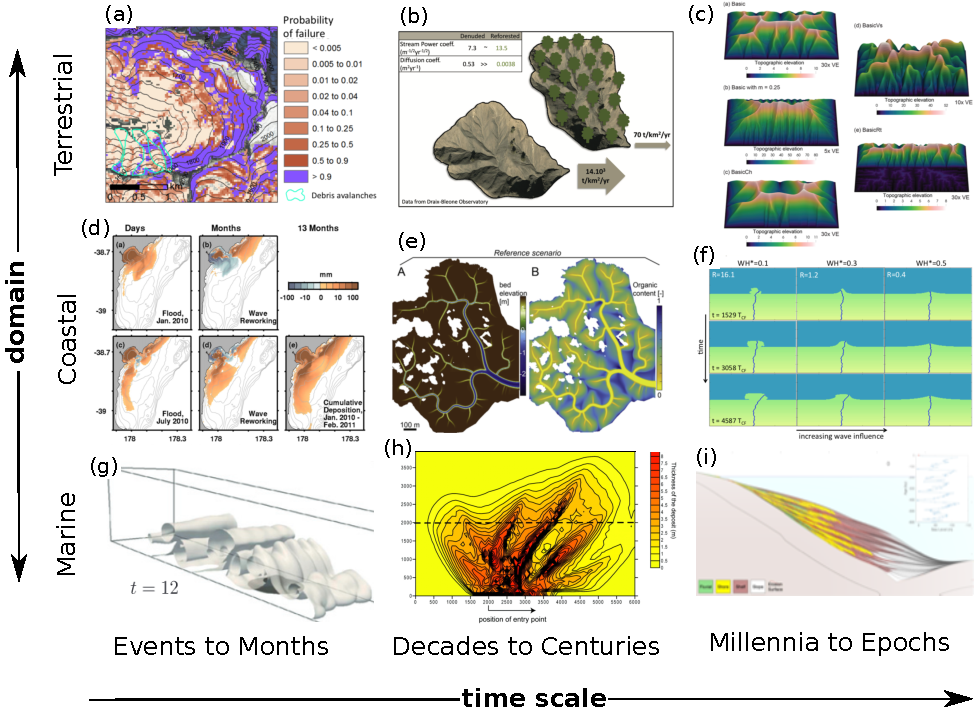
\includegraphics[width=6in]{Figures/model_examples.pdf}
\caption{Examples of Earth surface process models across a variety of domains and time scales, here focusing on models of sedimentary processes. (a) Probabilistic landslide occurrence \citep{strauch2018hydroclimatological}. (b) Catchment sediment yield \citep{carriere2020impact}. (c) Landform evolution \citep{barnhart2019terrainbento}. (d) Coastal and shelf dispersal of fluvially derived sediment \citep{kuehl2016source}. (e) Salt marsh evolution under tidal and sea-level forcing \citep{mariotti2018marsh}. (f) Delta evolution as a function of river and wave forcing \citep{ratliff2018exploring}. (g) Turbidity current dynamics \citep{nasr2013polydisperse}. (h) Submarine turbidity fan stratigraphy \citep{groenenberg2010flow}. (i) Sequence stratigraphy \citep{steckler2019developing}.}
\label{fig:modelexamples}
\end{figure}


Within the sphere of computing, numerical modeling---defined here as the computing of solutions to a set of equations and algorithms that represent a system---plays a central role. The process of formulating a computational model and the theory behind it encourages deep and precise thinking \citep[e.g.,][]{guest2020computational}. Computational models both encapsulate theory, and provide machinery with which to explore the consequences of that theory. \citet{pipitone2012assessing}, for example, described climate models as `executable theories of climate.' Numerical models in Earth and environmental science embody executable theory for many different aspects of the natural world (Figure~\ref{fig:modelexamples}). At the same time, the numerical algorithms and software that implements them provide a kind of mind-enhancing machinery. Whereas other scientific technology extends our senses---allowing us to `see' what lies beyond the visible spectrum, and to `feel' the vibrations in the Earth---computational modeling extends our cognitive capacity. By turning ideas into algorithms, we gain the ability to explore the logical consequences of our ideas, make predictions, and compare them with observations. Discovery comes not only when the calculations provide self-consistent explanations for otherwise mysterious phenomena, but especially when the calculations surprise us, revealing a logic trail that leads to new insights \citep{bras2003six}.

%Computing also converts primary observations from instruments or experiments into data that we can use. In remote sensing, for example, computational algorithms turn raw binary information (environmental data records) into measurements of topography, land cover, vegetation properties, and any number of other attributes. This kind of data processing is a form of modeling: applying a theory (often statistical) to a set of numbers in order to map or otherwise estimate a phenomenon of interest. More generally, software today forms a key piece of sustainable data management, sharing, and reuse \citep[e.g.,][]{hsu2015data}.%

With the rapid growth in computing and digital infrastructure, many scientists now devote a large fraction of their research time to developing software \citep{hannay2009scientists,prabhu2011survey,wilson2014best,singh2016unsung,pinto2018scientists}. A survey of nearly 2000 researchers in 40 countries by \citet{hannay2009scientists} revealed that 84\% of respondents considered software development important for their research. According to their findings and those of \citet{prabhu2011survey} scientists spend as much as a third of their time writing and debugging computer programs. In the geosciences  software has become critical research infrastructure: as vital and worthy of maintenance as ships, telescopes, and seismographic arrays. Yet the invisibility of software  has led to challenges in developing and sustaining this critical research infrastructure \citep{eghbal2016roads}.


\subsection{Growing pains}

Experimental science absolutely depends on having high-quality laboratory infrastructure, and operating it with careful, systematic protocols. In this respect, computational science differs only in the invisibility of its primary infrastructure. Experimental research methods, with their emphasis on transparency and replicability, pre-date computational science by over 200 years \citep{wilson2006s,fomel2009reproducible}, and so it comes as no surprise that computational science has experienced growing pains. Errors in software can have serious consequences for research. Software faults led to the failure of the Arianne rocket in 1996, and of the Mars Climate Orbiter mission in 1999. In 2006, discovery of a bug in image-processing software led to the retraction of five papers in computational biochemistry \citep{miller2006scientist}. High-profile cases like these have sparked concern about the quality and reliability of research software. Studies of scientific software development practices underscore these concerns, suggesting that the practice of formal testing of code correctness remains relatively limited \citep{post2005computational,wilson2006s,hannay2009scientists,nguyen2010survey,clune2011software,howison2011scientific,prabhu2011survey,kanewala2014testing,heaton2015claims}. \citet{hatton1997t} evaluated the performance of a collection of seismic data processing programs, and found that the results varied even among programs that claimed to use the same algorithm. Seeing little evidence of progress ten years later, \citet{hatton2007chimera} wondered whether the scientific community must `continue building scientific castles on software sands when we could do so much better?'

Serious flaws in scientific software are not inevitable, however. \citet{pipitone2012assessing} found, for example, that climate models, which are subject to rigorous testing and quality controls, have very low defect density as compared with other open-source software of similar scale. Their findings show that software quality control practices can work well when applied to research products. So why are such practices not used more widely? One common obstacle is simply a lack of awareness of, and training in, effective quality-control practices such as unit testing and continuous integration \citep{wilson2006s,faulk2009scientific,hannay2009scientists,kanewala2014testing}, a finding that led \citet{faulk2009scientific} to remark that `scientists are trained to manage threats to validity in experimental design but not in their codes.'

A related challenge lies in computational reproducibility: the ability to recreate the results of a study using the same data and software. The ability to reproduce others' findings forms a cornerstone of the scientific method. Yet as computational science has bloomed, concern has grown over the difficulty or impossibility of reproducing published results \citep[e.g.,][]{schwab2000making,peng2011reproducible,stodden2013setting,barba2016hard,alnoamany2018towards,chen2019open,krafczyk2019scientific}. In the words of \citet{leveque2009python}, `scientific and mathematical journals are filled with pretty pictures of computational experiments that the reader has no hope of repeating.' In a reproducibility study of 306 articles in the Journal of Computational Physics, \citet{stodden2018enabling} found only six that provided enough method information to re-run the analysis without help from the original authors. Of the remaining papers, about half were impossible to reproduce even after contacting the authors for assistance.

Reproducibility has several dimensions: sharing (the digital artifacts need to be available), discoverability (one needs to be able to find them), learnability (there needs to be sufficient documentation), and operability (the operating interface needs to be familiar, and the correct compute environment and dependencies must be available). Failure in any of these dimensions hurts productivity, because researchers end up spending more time either figuring out opaque, poorly documented software, or reinventing their own version from scratch. Collectively, reports of unreproducible results and unsustainable, under-tested software suggest that computational science relies on a brittle cyberinfrastructure, and productivity suffers as a result \citep{wilson2006s,faulk2009scientific,prabhu2011survey}.

A variety of factors contribute to the challenges of research software quality, reproducibility, and reusability. Most scientists lack formal training in software development, and tend not to know about tools and practices that could increase their productivity \citep{kelly2007software,basili2008understanding,faulk2009scientific,hannay2009scientists,hwang2017software,alnoamany2018towards,pinto2018scientists,kellogg2018role}.  Incentives also play a role: the academic system rewards publication of new results rather than production of high-quality, reusable software (though credit mechanisms for software are now starting to emerge) \citep{leveque2009python,howison2011scientific,morin2012shining,turk2013scaling,ahalt2014water,poisot2015best,hwang2017software,wiese2019naming}. The combination of incentive structure and lack of training in best practices can lead to inflexible, hard-to-maintain software \citep{brown2014run,johanson2018software}. Often enough it ends up as `abandonware' when a project ends \citep{barnes2010publish}. Reluctance by code authors to provide \textit{pro bono} support also plays a role. A certain embarrassment factor may contribute: in our own experience, as well as reports from other fields, researchers often express reluctance to share `messy' code, even when they have used the software as the basis for published research \citep{barnes2010publish,morin2012shining,leveque2013top}.



\subsection{New community practices}

Despite the growing pains, there are solutions on the horizon. Tools and practices already exist that can improve the quality and efficiency of software cyberinfrastructure, and improve productivity through coordination and reuse. Practices, tools, and techniques that the software community uses routinely have begun to see uptake in the sciences, with good success \citep{bangerth2013makes,turk2013scaling,hastings2014ten,wilson2014best,brown2014run,poisot2015best,hwang2017software,nanthaamornphong2017test,scott2017esip,taschuk2017ten,wilson2017good,benureau2018re,bryan2018excuse,adorf2018professionally,lathrop2019introduction}; in Section~\ref{sec:csdms}, we describe how the CSDMS community has implemented some of these. And while there remains a critical need for teaching and training in scientific computing, some universities, as well as community organizations such as Software Carpentry and various domain-centered groups (including CSDMS) have begun to fill that niche \citep[e.g.,][]{jacobs2016experiences}. 

One promising development is the emergence of software journals, which provides a mean to reward research software with the academic credit it deserves. For example, the Journal of Open Source Software (JOSS), which began publishing in May 2016, focuses not on papers about results obtained by software, but instead on the `full set of software artifacts' \citep{smith2018journal}. Reviewers of JOSS submissions evaluate the software directly; a one or two page abstract describing the purpose and function of package forms the only textual component, apart from documentation. For the Earth and environmental sciences, JOSS now complements more traditional text-based journals, such as Geoscientific Model Development, that provide a forum for software-oriented issues such as algorithm development and model verification. The growing importance of software in research has also led to a new type of career track: Research Software Engineers (RSEs), whose cross-training in computing and domain science positions them to help researchers build and maintain high-quality, sustainable software \citep{baxter2012research}. Thus, the academic world now has the beginnings of a credit mechanism that incentivizes high-quality research software cyberinfrastructure, and the first glimmers of a professional structure to help create and maintain that cyberinfrastructure. 

Better incentives and support for writing, documenting, and publishing research software can help address the productivity problem because they encourage software reuse over reinvention. Community software libraries and modular frameworks provide another avenue for reuse. Libraries are already widely available for general tasks such as numerical computing, parallel programming, and general science and engineering operations; some examples include PETSc \citep{abhyankar2018petsc}, Deal.II \citep{bangerth2007deal}, and the SciPy family \citep{2020SciPy-NMeth}. `Librarization' of software makes it easier to share, reuse, and maintain \citep{brown2014run}. Frameworks are defined as a collection of interoperable modules together with an environment for running and combining them. A framework provides a way to create coupled numerical models, and more generally to simplify computational workflows \citep[e.g.,][]{leavesley1996modular,voinov2004modular,peckham2013component}. Frameworks, as well as some open-source libraries, take advantage of contributions from many different community members: the software becomes a resource created by and for a scientific community. Growth of a community framework does not happen by accident, however. Case studies of community frameworks, libraries, and other software packages reveal that success requires two elements: a thoughtful, deliberate approach to community engagement \citep{bangerth2013makes,turk2013scaling,lawrence2015science}, and carefully designed standards and protocols \citep{peckham2013component,harpham2019introductory}.

\section{A Community-Based Modeling System for Earth-Surface Processes}
\label{sec:csdms}

The opportunities and growing pains that face scientific computing generally also apply to the sciences that deal with the Earth's surface. To embrace these opportunities, the CSDMS Integration Facility was launched in 2007 with a mission to accelerate the pace of discovery in Earth-surface processes research. The centerpiece was envisioned as `a modeling environment containing a community-built, freely available suite of integrated, ever-improving software modules aimed at predicting the erosion, transport, and accumulation of sediment and solutes in landscapes and sedimentary basins over a broad range of time and space scales' \citep{anderson2004community}. A key concept is that a modular, community-built modeling system not only opens new opportunities for using coupled models to explore the interactions among processes that were once considered in isolation, 
but also increases productivity by lowering the kinds of barriers described earlier. Achieving this requires a combination of:
\begin{itemize}
\item
\textbf{Community}: coordination, sharing, communication, collaboration (e.g., conferences, workshops, hackathons);
\item
\textbf{Computing}: software tools, standards, templates, access to high-performance computing and cloud resources;
\item
\textbf{Education}: in-person and online resources for learning tools, techniques, and best practices; resources for teaching these to others.
\end{itemize}
In the following sections, we describe the software technology, community building, and education elements developed by CSDMS, and how they help mitigate the obstacles discussed in Section~\ref{sec:background}. A useful way to understand the purpose of these products and activities is to consider the different modes in which researchers operate numerical models, and the opportunities that these different modes present to increase efficiency and productivity.


\section{A Taxonomy of Model Operation}
\label{sec:taxonomy}

What tasks are often required in computational modeling? And how might those tasks be made efficient? Here we identify six types of model-related activity, each of which has a unique set of challenges. Inspired by Bloom's Taxonomy of cognitive learning tasks, these six activities are arranged in order of complexity. The six modeling modes are summarized in Figure~\ref{fig:taxonomy}.

%The word `model,' whether used as a noun or a verb in a science and engineering context, has many different shades of meaning \citep[e.g.,][]{bras2003six}. Here we use the term \textit{mathematical model} to mean a set of equations and/or algorithms that represents a natural and/or engineered system. A \textit{numerical model} is a set of algorithms that implement a numerical solution (often approximate rather than exact) to a mathematical model, given a set of inputs. A \textit{model program} or \textit{model code} is a set of computer instructions, written in a programming language, that implements a numerical solution or algorithm. A single model code might provide the user with several different options for mathematical models or numerical algorithms. Conversely, a distinct model code might be designed to operate as a component in a larger coupled model, rather than as a stand-alone program, as with the component-based approach that we discuss here. Here, the word `model' by itself generally refers to a model program(s), including any scripts used for pre- or post-processing, analysis, visualization, etc. A model program can range in complexity from a simple short script to a multi-featured software package or library containing tens of thousands of lines of program code.%



% Requires the booktabs if the memoir class is not being used
% \begin{table}[htbp]
%   \centering
%   \topcaption{Taxonomy of Numerical Modeling Tasks} % requires the topcapt package
%   \begin{tabular}{>{\centering\arraybackslash}p{6in}} % Column formatting, @{} suppresses leading/trailing space
%       \toprule
%       {\centering BUILD} \\
%       Write a new numerical model program.\\
%       Debug and test.\\
%       \midrule
%       COUPLE \\
%       Iteratively exchange data and execute two different model programs or components. \\
%       May involve independent iteration (`loose coupling') or simultaneous solution to coupled set of equations (`tight coupling') \\
%       \midrule
%       MODIFY \\
%       Modify source code to change or enhance what the model does. \\
%       \midrule
%       LINK \\
%       Feed the output(s) of one model as input(s) to another in a sequential (one way) workflow.\\
%       \midrule
%       APPLY \\
%       Apply an existing program to a new problem or situation.\\
%       Usually requires configuring new inputs.\\
%       \midrule
%       REPRODUCE \\
%       Run a model program with pre-established inputs in order to learn a principle, demonstrate operation, or reproduce a known result.\\
%       Requires knowing how to operate the program and inspect the output.\\
%       \bottomrule
%   \end{tabular}
%   \label{tab:taxonomy}
% \end{table}

\begin{figure}[h!]
\centering
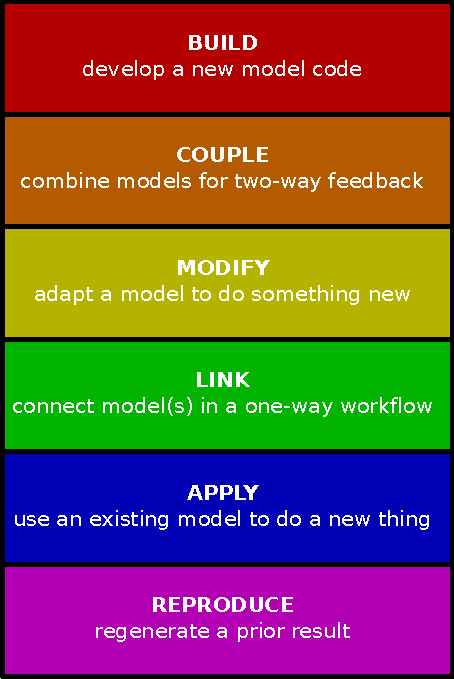
\includegraphics[scale=0.8]{Figures/model_operation_taxonomy.pdf}
\caption{Taxonomy of model operation tasks.}
\label{fig:taxonomy}
\end{figure}


\subsection{Reproducing}

The most basic operation of a numerical model is to run it with predefined inputs. This is often the first step in learning how to use a particular model. The ability to reproduce a model calculation efficiently involves all four of the FAIR principles \citep{wilkinson2016fair}. The user must be able to find and access the right version of the software. The user needs to learn how to execute the model: a task made easier if the program follows an interoperability standard. In order to reproduce the prior calculation, the user must have access to the input data, and must be able to recreate a compatible execution environment, including whatever dependencies might be needed.

\subsection{Applying}

To use a computational model in a new application, a user needs to understand the theory and algorithms behind it, and that requires good documentation. In addition, operating the model involves creating new input data, and often executing various pre-processing operations to derive the right kind of inputs. Sometimes it also requires setting up a grid mesh. In some cases, mesh generation is a major undertaking, for example, meshes for 2D storm-surge models such as ADCIRC \citep{luettich1992adcirc} and 3D regional ocean circulation models such as ROMS \citep{shchepetkin2005regional} are time-intensive to set up.


\subsection{Linking}

Here \textit{linking} means operating a model as part of a sequential workflow. For example, the workflow might include pre-processing data, using those data as input to the execution of a model, and using the output as input to another model, and/or performing additional operations on the model's output. To link a model in this way requires, among other things, compatibility in data formats. Any incompatibility between the outputs from one step and the inputs to the next means someone has to write code to do the appropriate translation.

\subsection{Modifying}

When a model provides most but not all of the functionality needed for a particular application, the would-be user faces a choice: modify the existing program, or write a new one that fits the purpose. Modifying an existing model program can save a lot of duplication of effort, but only when the model package includes good internal documentation, a modular design, and a structure that allows for modifications and enhancements while preserving the original functionality. A standard interface design can help by providing a familiar structure.

\subsection{Coupling}
% Let's be more broad and show some exciting coupling processes/domain research work spanning the larger community with some added references here. Examples: Julia Moriarty's paper are model coupling between domains https://bg.copernicus.org/articles/14/1919/2017/, Muriel Bruckners eco-sed interactions: https://agupubs.onlinelibrary.wiley.com/doi/full/10.1029/2019JF005092, Uwe Best, saltmarsh routines with Delft3D https://www.sciencedirect.com/science/article/pii/S1364815217309428, coasts and costs William's, https://agupubs.onlinelibrary.wiley.com/doi/full/10.1002/jgrf.20066, Lei Zhengs permafrost-hydrology, https://agupubs.onlinelibrary.wiley.com/doi/abs/10.1029/2019JF005060, Becca Lauzon's deltaRCM and sea ice, https://agupubs.onlinelibrary.wiley.com/doi/abs/10.1029/2019GL082792, hurricanes and flood inundation, http://dx.doi.org/10.26153/tsw/11477

Many of the exciting research frontiers in Earth and environmental science lie at the seams between systems. Some examples include: rivers and coasts \citep[e.g.,][]{ratliff2018exploring}; tectonics and Earth-surface processes \citep[e.g.,][]{roy2016dynamic}; ecosystems, soils, and landscape evolution \citep[e.g.,][]{istanbulluoglu2005vegetation,pelletier2017way,lyons2020speciesevolver}; permafrost and hydrology, and human actions and biophysical systems \citep[e.g.,][]{robinson2018modelling}. For these sorts of problem, coupled numerical modeling provides a great way to develop insight and to test hypotheses by comparing models with observations. The complexity of the task of coupling two numerical models depends on the nature of coupling (for example, sequential execution within each time step, versus coupling via joint matrix inversion) and on the program structure of each. The task becomes much simpler when both models offer a public, standardized interface: a set of callable functions that allow the appropriate exchange of data and mutual execution of algorithms.

\subsection{Building}\label{sec:build}

New ideas stimulate the need for new models. It is a healthy sign of growth when a scientific community produces lots of new models, because it signifies rapid development and exploration of new concepts. Writing a numerical model program from scratch can be a time-consuming exercise. Libraries of pre-existing functions and data structures can greatly simplify the task. Most modern programming languages offer libraries to handle basic mathematical operations, but even with these available, model-building can be a major effort. 

The job becomes easier when the developer can draw on component libraries that provide data structures and algorithms to address common tasks in numerical modeling, such as grid setup and input/output. It becomes easier still when common domain-specific algorithms have been librarized and made available as building blocks with a standard interface \citep[e.g.,][]{brown2014run}. Below we will look at an example of a component library that was designed specifically for building numerical models.



\section{The CSDMS Model Repository: A Platform for Sharing and Archiving Software Resources}
\label{sec:repo}

Not so long ago, making model source code freely available was more the exception than common practice. Model developers tended to view their models as trade secrets. If others wanted to use a model, the developer needed to be contacted, and could negotiate to become more involved in the research. Furthermore, fewer tools and platforms were available to promote sharing, like GitHub (established 2008) or SourceForge (established 1999).

Science clearly benefits from openly shared source code. For one, sharing reduces duplication. After all, there is less need to write a model from scratch, once a model has proven to capture a certain process well. Therefore, sharing of source code accelerates science, as others are on a faster trajectory to learn from and build upon previous model development efforts. Sharing of source code also makes science more robust and trusted, as people can report and fix bugs. Reproducing computational results requires shared source code. It is therefore encouraging to see a modeling culture shift over the last two decades \citep[e.g.,][]{hsu2015data}. For good data management, there are now the FAIR principals ---Findability, Accessibility, Interoperability, and Reusability---that have been formulated as guidelines for data producers and publishers \citep{wilkinson2016fair}. According to the FAIR principles, each dataset should have a unique digital object identifier (DOI) to get to the data, associated with searchable metadata. By including a formal, broadly applicable representation language, and using open and widely accepted domain-relevant vocabularies and ontologies, data sets become more interoperable. And by providing an abundance of documents that describe datasets and how they can be used, including license information, data become more reusable.

For model code, version-control platforms are now more widely used for sharing source code. But as the FAIR-data principles indicate, sharing code by itself is not enough. Therefore, CSDMS implemented the FAIR principles in setting up a model repository for Earth surface dynamics (Figure~\ref{fig:repo}). A minimal set of metadata parameters is defined to: describe a model, provide contact information for the model development team, indicate technical details such as operating platform and the software license, describe the model input and output, list its processes and key physical parameters, and indicate limitations. This minimal set of metadata includes a link to the actual source code, which needs to be made available 24/7 through a personal web repository, or through the CSDMS community repository. All model metadata stored on the CSDMS web server, as well as the actual source code (when stored in the CSDMS code repository on GitHub) are accessible for machines through web APIs. This makes it possible to automatically find and use the model. DOIs for stable versions of any listed code are generated on request and included with the metadata. Model metadata are enriched by including additional reference information, such a comprehensive bibliography. Following this practice, the CSDMS model repository currently holds 387 open source models of the community (as of Feb 2021). The models and tools in the repository span a range of languages, with Python, C, and Fortran being the most popular (Figure~\ref{fig:languages}). The diversity of languages raises a challenge in creating an interoperable framework. We will return to this point, and look at one solution, in Section~\ref{sec:babelizer}.

\begin{figure}[h!]
\centering
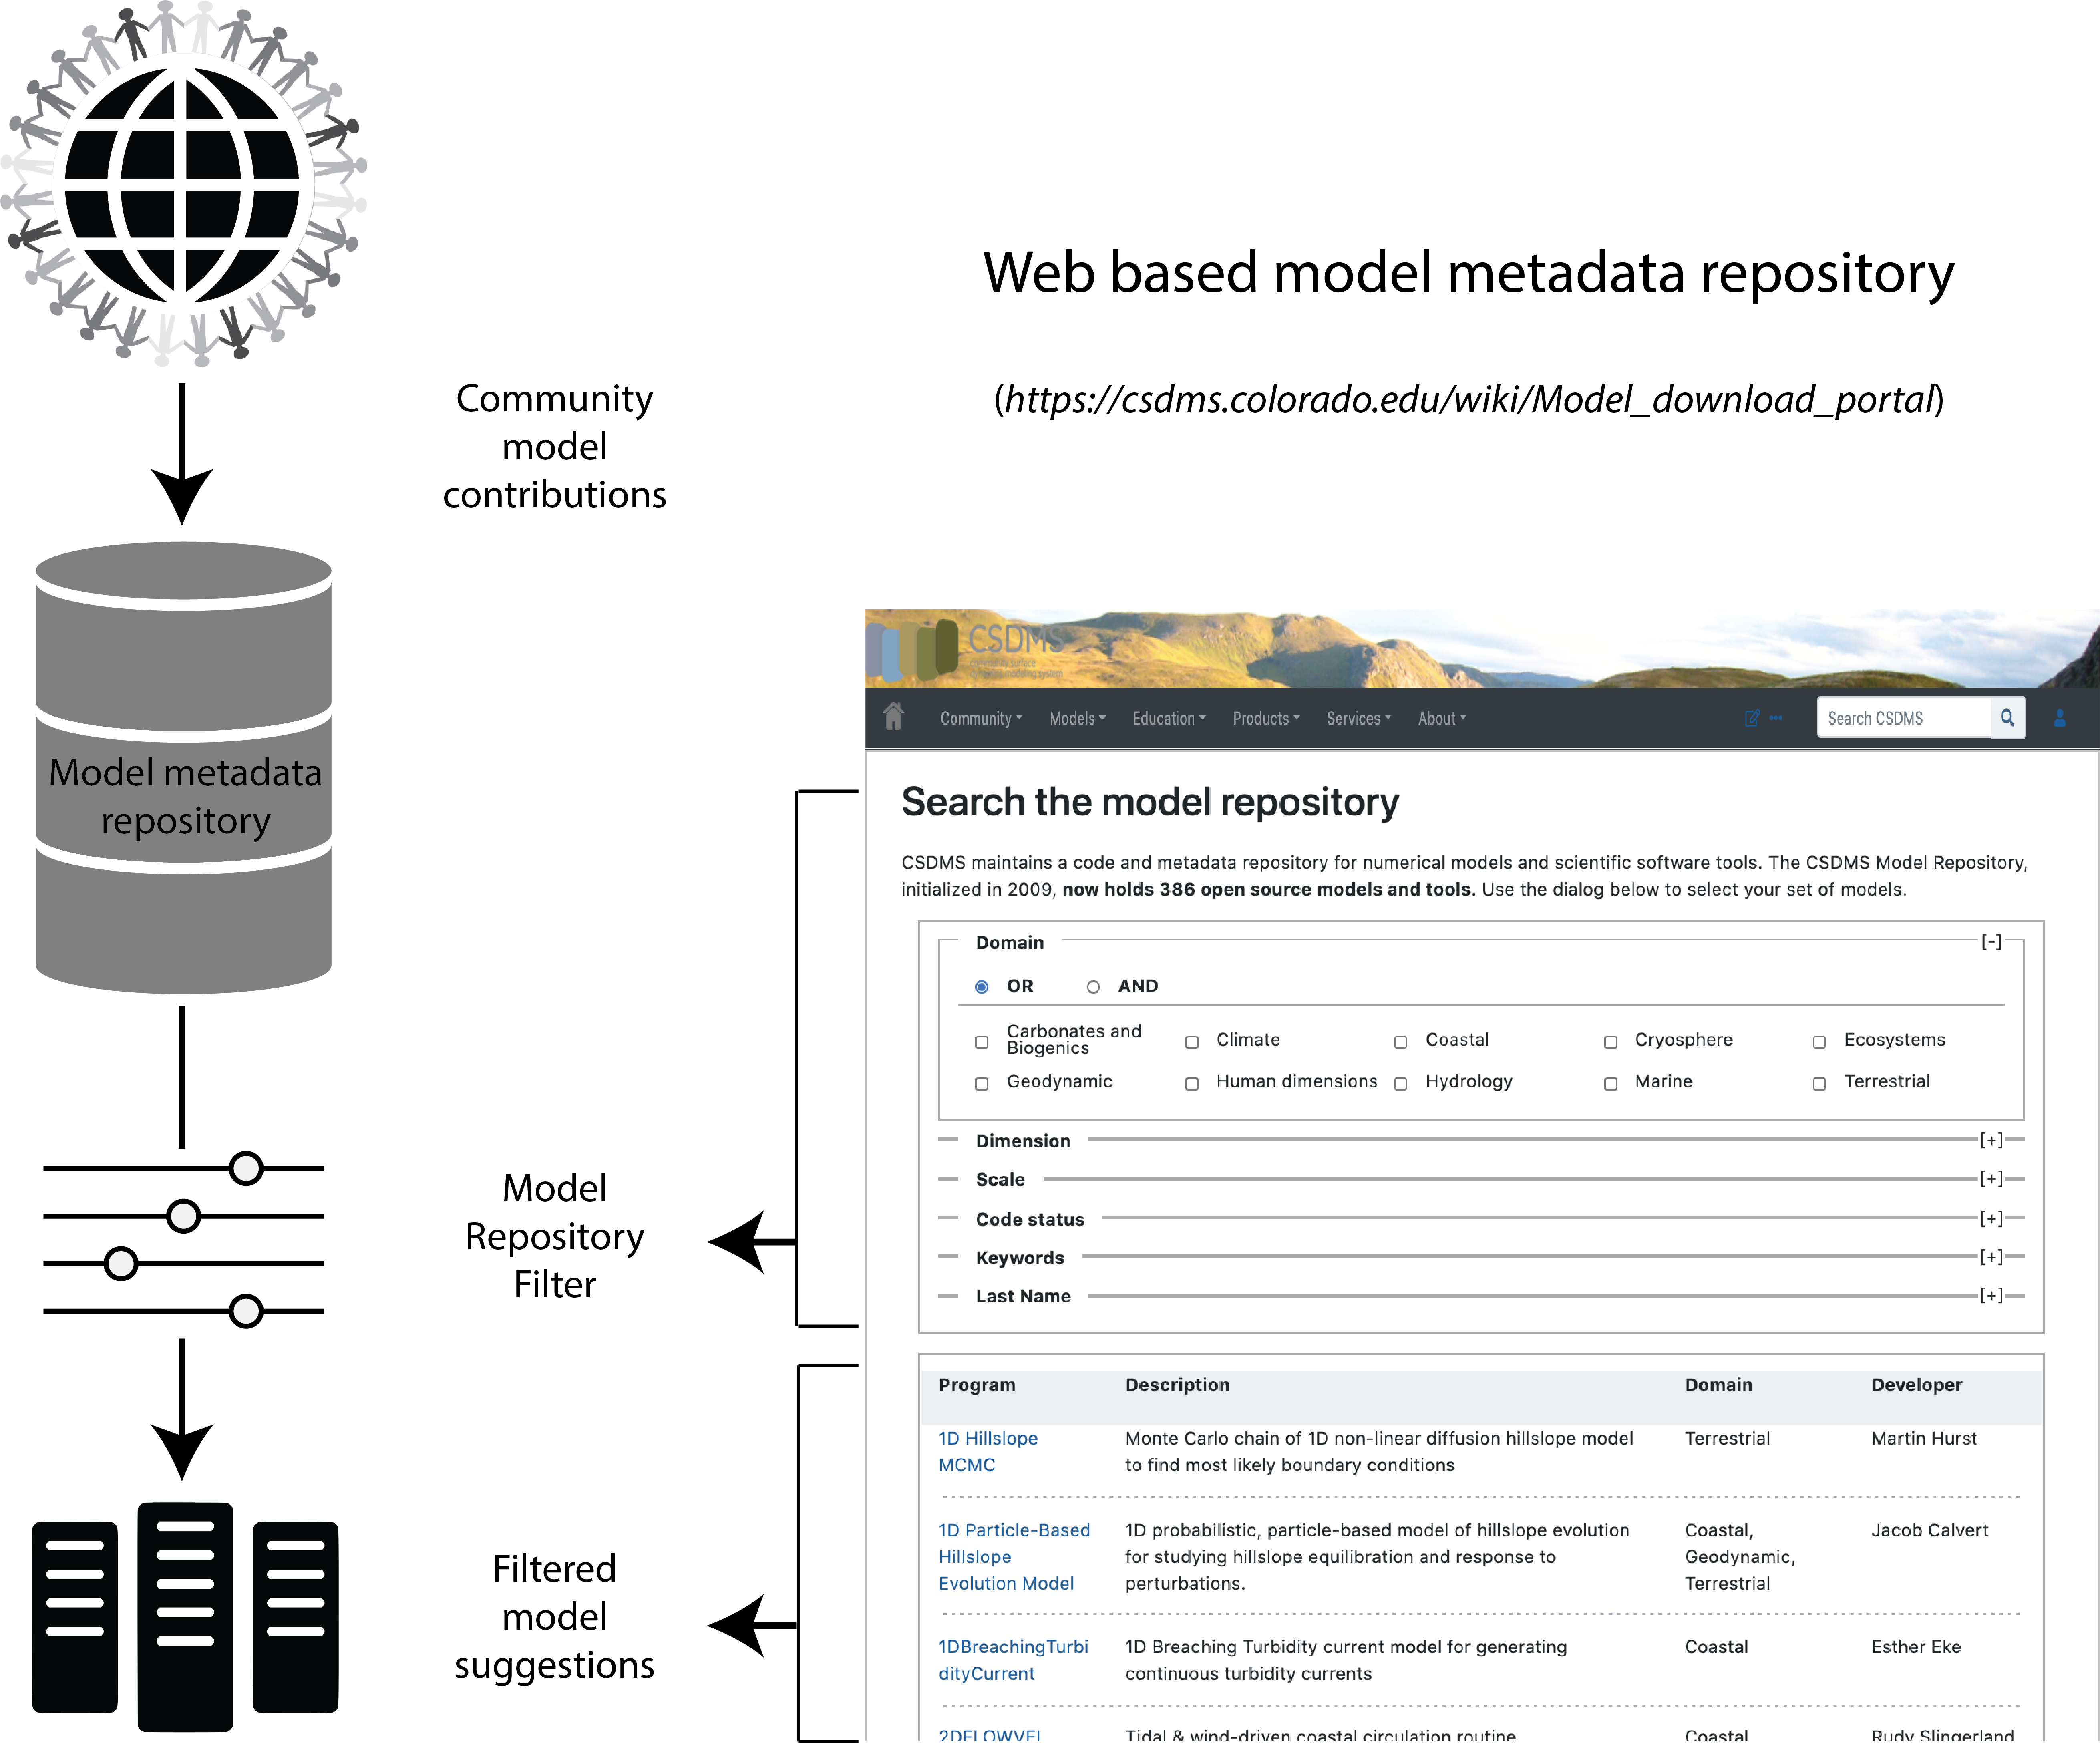
\includegraphics[width=5    in]{Figures/model_repository2.png}
\caption{The CSDMS Model Repository.}
\label{fig:repo}
\end{figure}



\begin{figure}[h!]
\centering
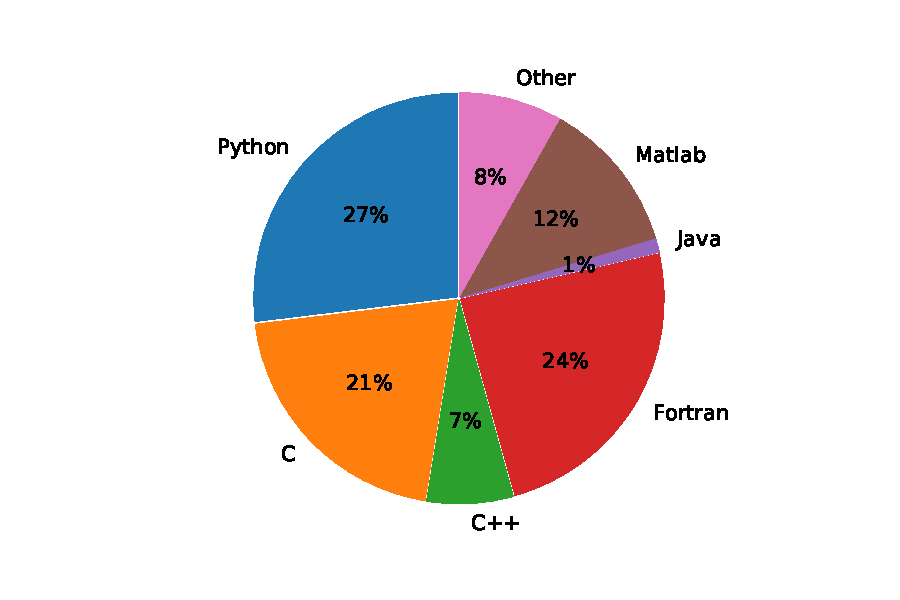
\includegraphics[scale=0.8]{Figures/languages_in_repository.pdf}
\caption{Distribution of different languages used by models and tools in the CSDMS Model Repository (percentages out of 453 total programs; not weighted by program size).}
\label{fig:languages}
\end{figure}


\section{The CSDMS Workbench}
\label{sec:workbench}

The \textbf{CSDMS Workbench} is a suite of tools, standards, documents, and resources that collectively provide a modular environment for model execution, analysis, and model-data integration. The Workbench comprises six main elements: 
\begin{enumerate}
    \item The \textbf{Basic Model Interface (BMI)}: an interface standard that simplifies model execution and coupling \citep{hutton2020basic,peckham2013component}.
    \item \textbf{Babelizer}: a language-bridging tool that adds a Python interface to BMI-enabled model programs written in various other languages.
    \item \textbf{pymt}: a Python-language execution and model-coupling environment, which includes utilities for grid mapping and other operations, together with a set of model components.
    \item \textbf{Data Components}: small Python-language modules that use the BMI to fetch data from particular data sets.
    \item \textbf{Landlab}: a component-based Python library for model building and sharing of interoperable components \citep{hobley2017creative,barnhart2020short}.
    \item \textbf{Standard Names}: An ontology standard for naming variables.
\end{enumerate}
In the following we give a brief description of each of these elements, and how they combine to form a modular modeling system.

\subsection{The Basic Model Interface (BMI) Standard}
\label{sec:bmi}

%- standardization: BMI

%(note: this isn't meant to be a substitute for the BMI papers; it's just a relatively short summary, probably with a table or figure, plus a figure illustrating an application in the literature or underway, e.g., Hoch et al. (2017) and/or PRMS)

% Outline:
% 1. Intro to idea of BMI (use Greg's intro to BMI docs
% 2. Description of BMI methods
%   a. Include table
%   b. Include sample code
% 3. Example of BMI use in research (I like Greg's suggestion of Hoch paper)
%   a. Include figure

When you sit in the driver's seat of an unfamiliar car,
you're presented with a familiar sight:
whatever the make or model,
the vehicle provides
a steering wheel, brake pedal, and speedometer.
%along with other controls and readouts
%that are common to essentially all cars on the planet.
Although we don't usually think of it this way,
drivers across the globe benefit
from a \textit{standard interface}---a set of control mechanisms and information displays
that have %basically
essentially the same design
regardless of whether the car
is a tiny electric two-seater or a giant stretch limousine.
This standard interface makes operating a car much easier
than if each vehicle presented a radically different interface.
Imagine a world where switching from a sports car to a pickup truck
required months of study and practice!

We believe %that
numerical models should offer a similar standardization.
To this end, CSDMS
developed the Basic Model Interface (BMI) \citep{peckham2013component,hutton2020basic}.
%a set of standard control and query functions for models.
In software engineering,
an interface is a named set of functions
with prescribed arguments and return values.
The BMI provides a standard set of functions
for querying and controlling a model.
Just as with a car,
when a model is equipped with a BMI,
it becomes easier to use
because its control functions are now the same as every other model with a BMI.

Further, because BMI includes variable-exchange functions,
a model with a BMI can be coupled with other models that expose a BMI.
Table \ref{tab:bmi} lists the individual functions
that comprise the Basic Model Interface,
along with a brief description of each.
The table shows the current version of BMI, version 2.0,
which represents a collection of improvements to the original specification,
especially in the representation of model grids \citep{hutton2020basic}. A model program that has been \textit{wrapped} with a BMI can function as an interoperable \textit{component}, which can be combined with others to create integrated models (Figure~\ref{fig:component}).

\begin{table}[htbp]
    %\Small
    \topcaption{Listing and description of Basic Model Interface (BMI) functions.}
    \begin{tabular}{ll}
        \hline
        Function Name &
        Description \\
        \hline\hline
        
        \verb|initialize| & Perform startup tasks for the model. \\
        \verb|update| & Advance model state by one time step. \\
        \verb|update_until| & Advance model state until the given time. \\
        \verb|finalize| & Perform tear-down tasks for the model. \\
        \verb|get_component_name| & Name of the model. \\
        \verb|get_input_item_count| & Count of a model’s input variables. \\
        \verb|get_output_item_count| & Count of a model’s output variables. \\
        \verb|get_input_var_names| & List of a model’s input variables. \\
        \verb|get_output_var_names| & List of a model’s output variables. \\
        \verb|get_var_grid| & Get the grid identifier for a variable. \\
        \verb|get_var_type| & Get the data type of a variable. \\
        \verb|get_var_units| & Get the units of a variable. \\
        \verb|get_var_itemsize| & Get the size (in bytes) of one element of a variable. \\
        \verb|get_var_nbytes| & Get the total size (in bytes) of a variable. \\
        \verb|get_var_location| & Get the grid element type of a variable. \\
        \verb|get_current_time| & Current time of the model. \\
        \verb|get_start_time| & Start time of the model. \\
        \verb|get_end_time| & End time of the model. \\
        \verb|get_time_units| & Time units used in the model. \\
        \verb|get_time_step| & Time step used in the model. \\
        \verb|get_value| & Get a copy of values of a given variable. \\
        \verb|get_value_ptr| & Get a reference to the values of a given variable. \\
        \verb|get_value_at_indices| & Get variable values at specific locations. \\
        \verb|set_value| & Set the values of a given variable. \\
        \verb|set_value_at_indices| & Set the values of a variable at specific locations. \\
        \verb|get_grid_rank| & Get the number of dimensions of a computational grid. \\
        \verb|get_grid_size| & Get the total number of elements of a computational grid. \\
        \verb|get_grid_type| & Get the grid type as a string. \\
        \verb|get_grid_shape| & Get the dimensions of a computational grid. \\
        \verb|get_grid_spacing| & Get the spacing between grid nodes. \\
        \verb|get_grid_origin| & Get the origin of a grid. \\
        \verb|get_grid_x| & Get the locations of a grid’s nodes in dimension 1. \\
        \verb|get_grid_y| & Get the locations of a grid’s nodes in dimension 2. \\
        \verb|get_grid_z| & Get the locations of a grid’s nodes in dimension 3. \\
        \verb|get_grid_node_count| & Get the number of nodes in the grid. \\
        \verb|get_grid_edge_count| & Get the number of edges in the grid. \\
        \verb|get_grid_face_count| & Get the number of faces in the grid. \\
        \verb|get_grid_edge_nodes| & Get the edge-node connectivity. \\
        \verb|get_grid_face_edges| & Get the face-edge connectivity. \\
        \verb|get_grid_face_nodes| & Get the face-node connectivity. \\
        \verb|get_grid_nodes_per_face| & Get the number of nodes for each face. \\
    \hline
   \end{tabular}
   \label{tab:bmi}
\end{table}

While a BMI can be written for any language,
CSDMS currently supports four languages: C, C++, Fortran, and Python.
A simple example of using a BMI written in Fortran
is shown in Listing~\ref{listing:bmi_code} below.
%
% minted is super cool, nicer than just verbatim -MP
\begin{listing}[ht]
\topcaption{Example Fortran BMI code.}
\begin{minted}{fortran}
  type (bmi_prms_surface) :: model
  character (len=*) :: config_file
  integer :: status
  double precision :: now, end_time

  status = model%initialize(config_file)
  status = model%get_current_time(now)
  status = model%get_end_time(end_time)
  do while (now < end_time)
     status = model%update()
     status = model%get_current_time(now)
  end do
  status = model%finalize()
\end{minted}
\label{listing:bmi_code}
\end{listing}
%
The model shown in this example
is the surface water component of the Precipitation Runoff Modeling System (PRMS),
developed by the U.S. Geological Survey \citep{leavesley1984precipitation}.
In the example,
the model is initialized from its native configuration file,
then stepped forward in time until it reaches its stop time,
whereupon any resources it uses are deallocated.
Note that only BMI function calls are used to drive the model;
no knowledge of the underlying calls to control PRMS is needed.

\cite{hoch2019evaluating} provide a current research example of using BMI. 
In their study,
they coupled a hydrologic model, PCR-GLOBWB,
with a pair of hydrodynamic models, CaMa-Flood and LISFLOOD-FP,
through BMI.
They observed that a coupled model system
enhanced the accuracy of peak discharge simulations (Figure~\ref{fig:hoch_2019_fig6}).
%and improved representation of observed flood extent in flood maps
%(Figure 7 from their paper).
%
\begin{figure}[h!]
\centering
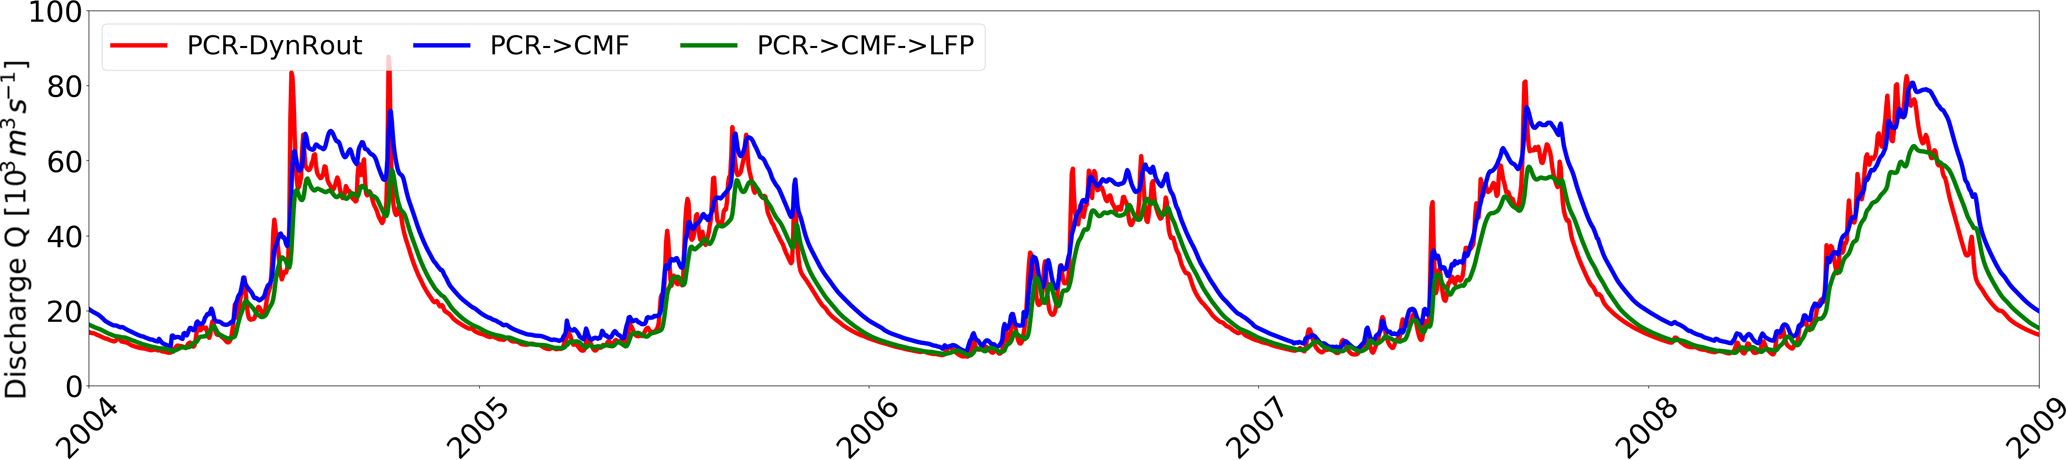
\includegraphics[scale=0.8]{Figures/nhess-19-1723-2019-f06.png}
\caption{Simulated discharge at a river monitoring station from coupled hydrologic and hydrodynamic models. (Reproduced from Figure 6 in \citet{hoch2019evaluating}.)}
\label{fig:hoch_2019_fig6}
\end{figure}
%
\citeauthor{hoch2019evaluating}\ conclude
that `results confirm that model coupling can indeed be a viable way forward towards more integrated flood simulations. However, results also suggest that the accuracy of coupled models still largely depends on the model forcing.'

\subsection{Language Interoperability: The Babelizer}
\label{sec:babelizer}

Looking at Figure~\ref{fig:languages},
we notice that software generated by the CSDMS community
reflects a range of programming languages and, so, language interoperability is critical
to a coupling framework if it is to bring together this diverse set of models.

One approach to solving this problem is to choose a \textit{hub} language through
which other languages will communicate. An advantage of this approach is that
it needs only to provide bridges from each supported language to the hub
language, rather than building bridges for each language to every
other language. CSDMS uses Python as a hub language for several reasons: it is open source, has a large user
base in the user community, has an active community that supports a vast library
of 3rd-party packages (numpy, scipy, xarray, pandas, etc.), and,
importantly, there are existing pathways to bring many other languages into Python.

The \textit{babelizer} is a command-line utility CSDMS created to streamline the
process of bringing a BMI component into Python. For libraries that expose a
BMI, the \textit{babelizer} creates the necessary glue code to create a Python
importable package that presents the BMI component as a Python class. We
wrote the \textit{babelizer} to be easily extensible to additional languages but,
presently, it can be used to wrap libraries written in C, C++, and Fortran
using the Cython language.


% refer to Figure~\ref{fig:languages} somewhere in this section

% - need a lingua franca; here, Python because of its popularity, num/sci libraries, and high-level interpreted nature

% - babelizer: tools and procedures to take BMI'd code in C, C++, F, (Julia??) and convert to Python-callable module



% - notion that the BMI specification makes it relatively straightforward to add a language (or should this go under BMI?)

\begin{figure}[h!]
\centering
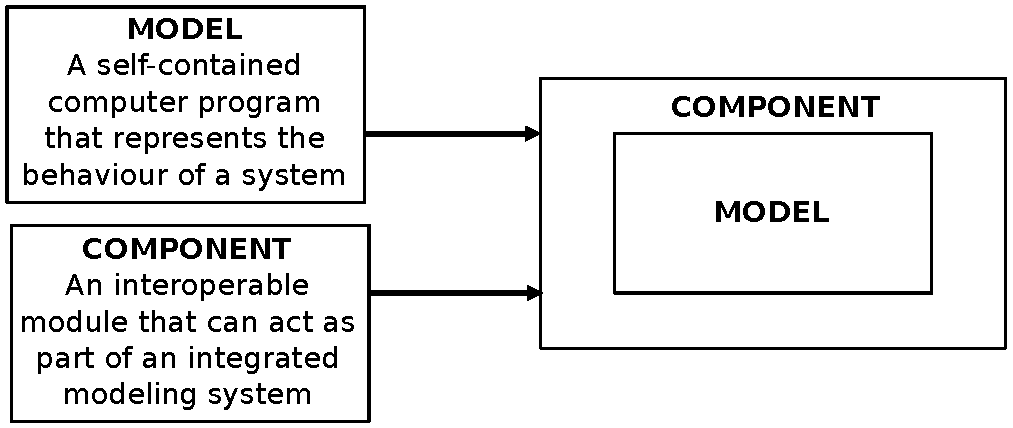
\includegraphics[scale=0.5]{Figures/model_to_component.pdf}
\caption{When a numerical model program is `wrapped' with a standard interface and compiled as an importable module, it becomes an interoperable \textit{component}.}
\label{fig:component}
\end{figure}


\subsection{Execution and Coupling Framework: pymt}
\label{sec:pymt}

Models in the Earth Sciences are as diverse as the environments they are intended to represent.
Codes are written by hundreds of authors, in different languages, from a diverse range of domains,
operate on time and space scales that span orders of magnitude,
and are oftentimes written in isolation---never intending to be used
by someone outside the core development team. And so, models do not fit so neatly together.

Although the CSDMS collection of models is incredibly diverse,
there is a common thread possible---the Basic Model Interface (BMI; Section \ref{sec:bmi})
---that connects them and allows us to
create tools that allow scientists to easily pick up, run,
and even couple these models with one another. While only a subset of codes in the Model Repository (Section~\ref{sec:repo}) provide a BMI, the concept is general enough that
any model can be given one. To provide a framework for operating and coupling these BMI-equipped codes, the CSDMS Integration Facility develops and maintains a Python package known as the \textit{pymt} 
(Python Modeling Toolkit).

\begin{table}[htbp]
    \topcaption{Models available as components in the Python Modeling Tool}
    %\Small
    \begin{tabular}{llc}
        \hline
        \textbf{Component} & \textbf{Property / Process(es)} & \textbf{Language} \\
        \hline
        FrostNumber & permafrost occurrence & Python \\
        Kudryavtsev (Ku) & soil active layer thickness & Python \\
        GIPL & soil temperature \& heat flow & Fortran \\
        ECSimpleSnow & snow balance & Fortran \\
        HydroTrend & river water \& sediment discharge & C \\
        RAFEM & river avulsion \& floodplain evolution & Python \\
        CHILD & landscape evolution & C++ \\
        CEM & sandy, wave-dominated coastline evolution & C \\
        GridMet & meteorological data access & Python \\
        Sedflux3D &  seafloor evolution & C \\
        Avulsion & river avulsion & C \\
        Plume & hypopycnal sediment plume& C \\
        Subside & 2D lithospheric flexure & C \\
        OverlandFlow$^*$ & Surface water runoff & Python \\
        Flexure$^*$ & 1D/2D lithospheric flexure & Python \\
        LinearDiffuser$^*$ & 2D linear diffusion & Python \\
        ExponentialWeatherer$^*$ & Weathering of bedrock on hillslopes & Python \\
        TransportLengthHillslopeDiffuser$^*$ & Hillslope diffusion & Python \\
        Vegetation$^*$ & productivity, biomass and leaf area index & Python \\
        SoilMoisture$^*$ & Root-zone soil moisture & Python \\
        DepthDependentDiffuser$^*$ & Depth and slope dependent linear diffusion & Python \\
        FaSTMECH & River flow and morphodynamics solver & Fortran \\
        PRMSStreamflow & River channel flow (Muskingum routing) & Fortran \\
        PRMSGroundwater & Subsurface water flow & Fortran \\
        PRMSSoil & Soil zone flow & Fortran \\
        PRMSSurface & Surface water flow & Fortran \\
        \hline
        \hskip1em (* = Landlab component) & \\
   \end{tabular}
   \label{tab:components}
\end{table}

The CSDMS Integration Facility has written the pymt as a Python package that gives
scientists a set of utilities for running and coupling Earth
System models within a Python environment. We see the pymt
as, primarily, two things:
(1) a collection of Earth-surface models, in which every model exposes
a standardized interface (and so, if you are able to run one model,
you will be able to run any model), and
(2) tools needed for coupling models across disparate time and space scales. 
A key feature of pymt is extensibility: any contributor can implement a BMI and use the babelizer (\ref{sec:babelizer}) to create to add a new model or utility to the toolkit.

Although the pymt itself is written in Python, the models in its
collection need not be written in Python. The babelizer allows developers and contributors to bring 
models from other languages into a Python environment. The current 
pymt model collection is detailed
in Table \ref{tab:components}. One thing to note when reading through
this list, apart from the diversity of models, is that models span a range of granularity (that is, the size of a model's scope). 
Granularity ranges from a single equation
(for example, from hydrology, the Richards equation or Green-Ampt method to model
infiltration) to a collection of coupled process models (or even
a complete modeling framework; e.g.\ \textit{CHILD} \citep{tucker2001channel} or \textit{Sedflux3D} \citep{hutton2008sedflux}). However, we find that the most useful
model size is one between these two extremes, which simulates a single physical process (for example the compaction of sediment under an overlying load, or the transport of sediment by way of hypopycnal sediment plumes). Models of this
size are flexible in the number of other models they can couple with but
not so small that they do not justify the extra overhead of creating a separate
component.


% The \textit{pymt} model collection contains a wide range of process models and data sets that include the ocean, coast, and land, as well as stratigraphic models. The range of model time and spatial scales, and granularity presents several problems when coupling these models
% (and data) with one another.

We have included with the pymt a collection of tools a modeler can use to
connect a disparate set of models. For example, models will not
necessarily operate on the same spatial grid and so may have different
spatial resolutions or even different grid types (e.g., raster versus 
unstructured mesh). To overcome this problem, we use
the Earth System Modeling Framework (ESMF) grid mapper, which uses interpolation to translate variables between grids. Using this grid
mapper, a modeler can write a script that gets grid values from
one model and pymt will automatically map them onto the grid of 
another (Figure~\ref{fig:child_sedflux}).

Another common issue when exchanging data between
models in a coupled is system is unit mismatches. To address this issue, the pymt contains a Python
wrapped version of the \textit{udunits} unit conversion library.
When connecting components within pymt, the user specifies
the units for quantities that components will either use or
provide. As with grid mapping, the pymt decorates the standard
BMI with additional functionality, thus leaving these common
tasks to the framework rather that to the developer of each model. 
The two quantity converters (grid mapping and
unit conversion) target the BMI \texttt{get\_value} methods, that is
differences in quantities defined on a spatial grid. However,
two models can also differ temporally.

Depending on a model's time resolution, the algorithm it uses
to solve a set of equations, or the time scale being simulated,
models may not advance forward time at compatible intervals.
However, when coupling models, we require the exchange of quantities
to be made when models are synchronized in time.  While the BMI
\texttt{update\_until} method could be used for this, we recognize
(for some of the reasons listed above) that not all models
can realistically implement this method. For such cases we've
added time interpolators to the pymt by way of a modified
\texttt{update\_until} method that estimates values at intermediate time
steps. The pymt accomplishes this by temporarily saving quantities
at previous time steps and then interpolating between time steps.
Consider, for example, a user who wants to couple two models:
the first advances in time at $\Delta t$ and the second
at a larger time step of $2 \Delta t$. Both models sit at time $t_0$ but the first
wants to get a quantity, $x(t)$, from the second at $t = t_0 + \Delta t$.
To do so, pymt advances the second model by its time step to $t = t_0 + 2 \Delta t$
and returns an interpolated value of $x(t_0 + \Delta t)$.
pymt does this behind-the-scenes within the second model's
\texttt{update\_until} method.

\begin{figure}[h!]
\centering
\includegraphics[scale=0.25]{Figures/child_sedflux.png}
\caption{Results of a coupling experiment using the Python Modeling Toolkit (pymt).
The CHILD model (C++; unstructured mesh) erodes an uplifting landscape and
transports sediment to the coast. Sedflux (C; structured rectilinear grid)
sends sediment from the coast to the ocean as surface plumes
where it then settles onto the seafloor. As sediment accumulates on the seafloor,
deltas begin to form and this new landscape is sent back to CHILD, completing the two-way coupling
between these two pymt components.}
\label{fig:child_sedflux}
\end{figure}


Figure \ref{fig:child_sedflux} shows the results of a coupling experiment
that demonstrates some of pymt's capabilities.
Here we have coupled the landscape evolution model CHILD with
the seascape evolution model sedflux3D. The landscape
is uplifted and eroded by CHILD, including fluvial transport of sediment to the coast. At the coast, sedflux3D takes over and transports sediment to the seafloor through surface sediment plumes and, over time, builds up a delta, which becomes part of
the subaerial landscape (and thus part of the domain of CHILD). For every time step, CHILD passes river fluxes
to sedflux3D which, in turn, passes updated landscape elevations back to CHILD.
Apart from the difference in domains (land vs.\ sea), the two models also differ in their computational grids: CHILD uses an unstructured mesh while sedflux3D uses a uniform rectilinear grid. The pymt manages the time stepping, variable exchange, and the mapping of variables between the two grids.

In addition to providing a set of coupling tools, pymt provides
an interactive environment to couple and run models. Although the two models in
our previous example were written in C (sedflux3D) and C++ (CHILD), when imported as Python classes in pymt, users are able to instantiate and 
run the two models interactively. A user advances models one time step at a time and can then
query or even change values dynamically. When run in their native languages, a user
would set the initial conditions for a model simulation and then let the model run
to completion before examining output. A user would never be able to dynamically change values as it advanced. The  functionality that pymt provides 
allows a user to experiment interactively, examining state variables
as the model evolves, and 
dynamically changing model state variables as it advances---all within a Python
environment with its large  collection of visualization and analysis packages.


\subsection{Data Components}

Researchers rarely use numerical models in isolation. Working with models nearly always includes working with data sets too: the data that go into a model as input, the output data that a model produces, and the data to which a model's output is compared (Figure~\ref{fig:taxonomy}). Productivity suffers when these data sets are cumbersome to access and use. Just as model interface standards like BMI make it easier to work with numerical models, standardized methods for data access and retrieval can ease the burden of working with data. To that end, CSDMS has developed a programmatic approach that uses the BMI for data retrieval and access. Functions such as \texttt{initialize()} retrieve and open a data set, and \texttt{get\_value()} fetches particular data items or subsets. A program that uses the BMI to access items from a particular data set is known as a \textit{Data Component}. Using the same interface for model and data operation makes it easier to swap models and data sets; for example, one might compare use of model-calculated versus measured wave heights in a simulation of coastal sediment transport. Because CSDMS Data Components are written in Python, they can take advantage of data-management packages like \texttt{pandas} and \texttt{xarray}.

The data components are designed to provide a consistent way to access various types of datasets (e.g., time series, raster grid, and multidimensional space-time data) and subsets of them without needing to know the original file formats. Each data component effectively `wraps' a dataset with a BMI (with the exception of certain BMI functions, such as \texttt{set\_value}, which do not apply to datasets). Data components can easily interact with BMI-enabled numerical models in the pymt modeling framework, or other similar frameworks.

One example is the National Water Model (NWM) data component. This data component can access and subset the forecasted streamflow time series generated by the NWM hydrologic modelling framework. Figure \ref{fig:data_component1} shows an example of how the NWM data component can be used to get the streamflow data at a river channel for a flooding event. Figure \ref{fig:data_component2} shows the corresponding time series plot. This data component includes a set of standard control and query functions (e.g.,  \texttt{initialize()}, \texttt{update()}). These standard methods make the dataset easier to couple with BMI-enabled numerical models  without needing to know the time-series file format.

\begin{figure}[h!]
\centering
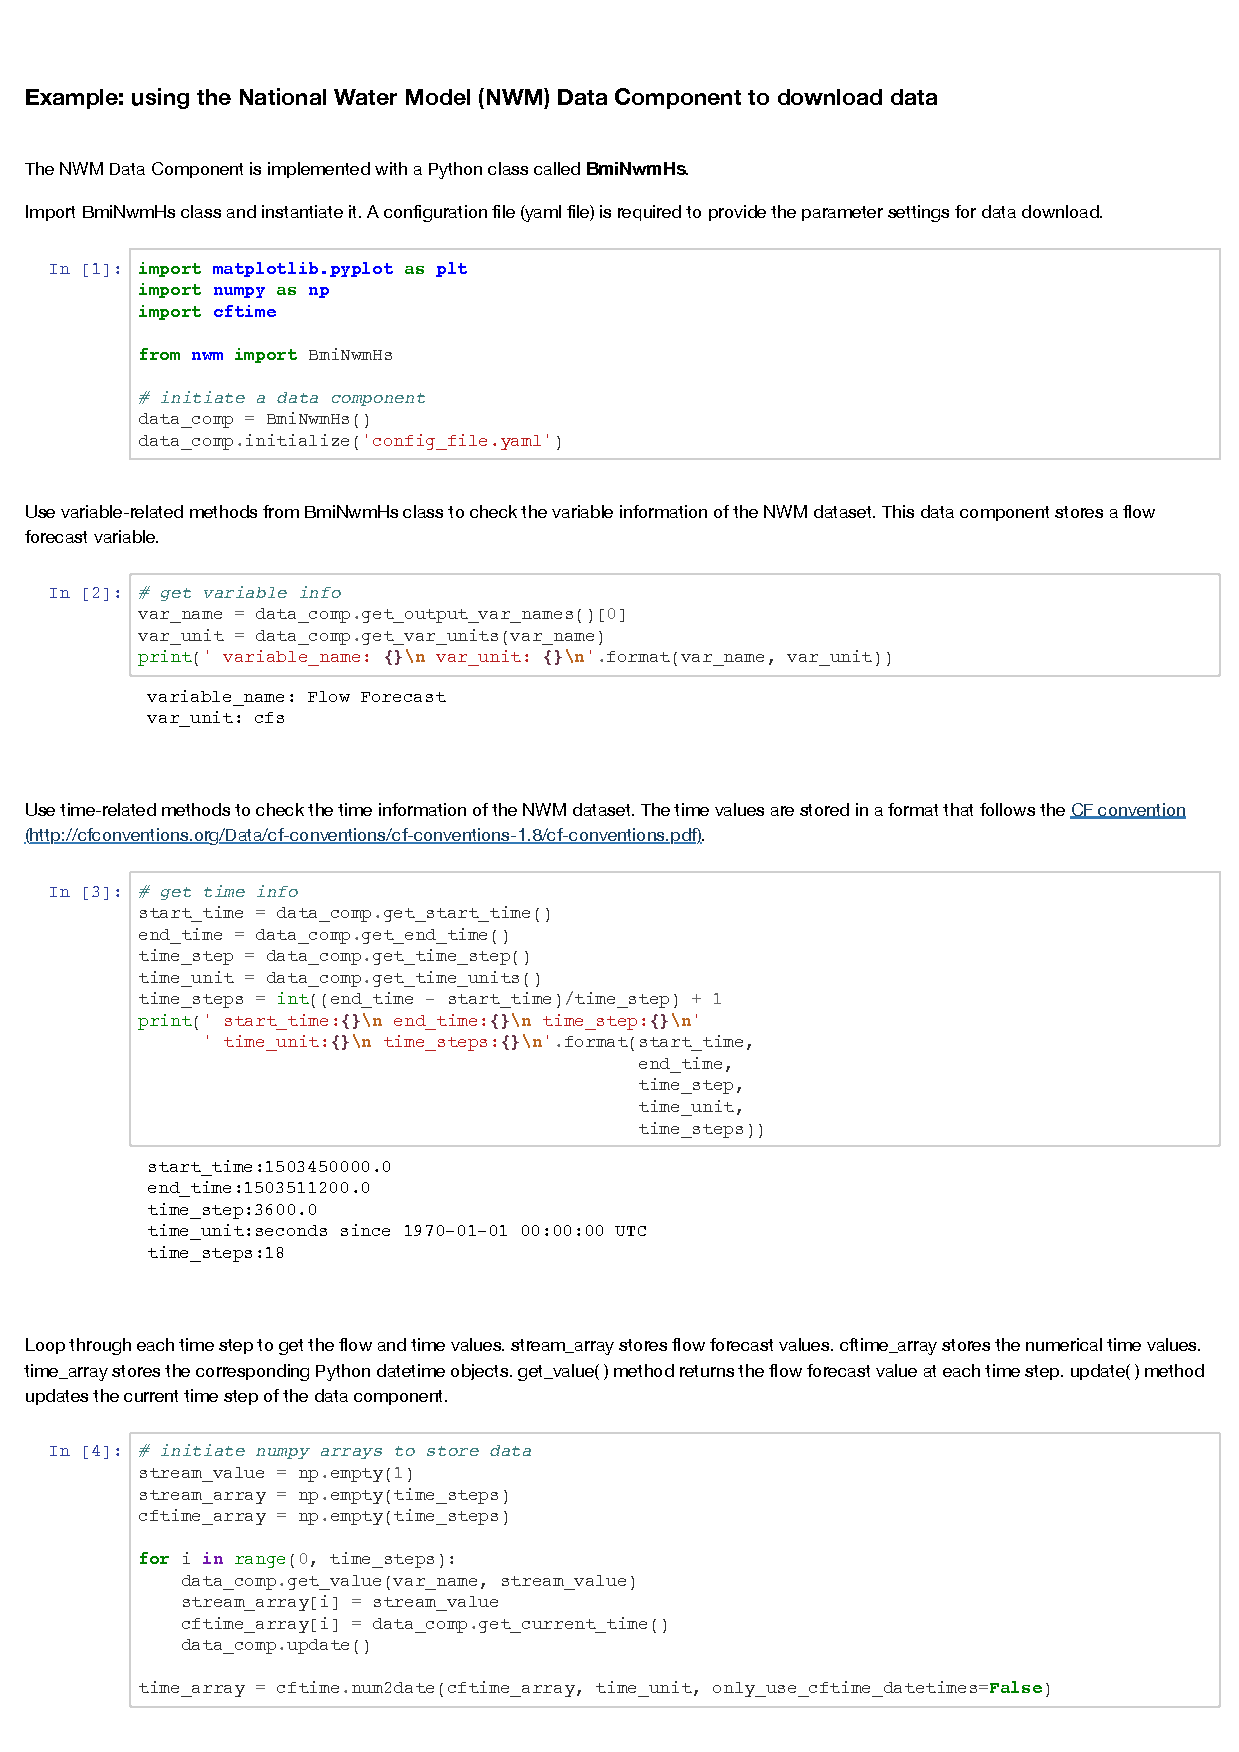
\includegraphics[scale=0.57]{Figures/nwm_example_latest.pdf}
\caption{Screenshot of a JupyterNotebook demonstrating how to use the NWM Data Component to access and subset a streamflow dataset. }
\label{fig:data_component1}
\end{figure}

\begin{figure}[h!]
\centering
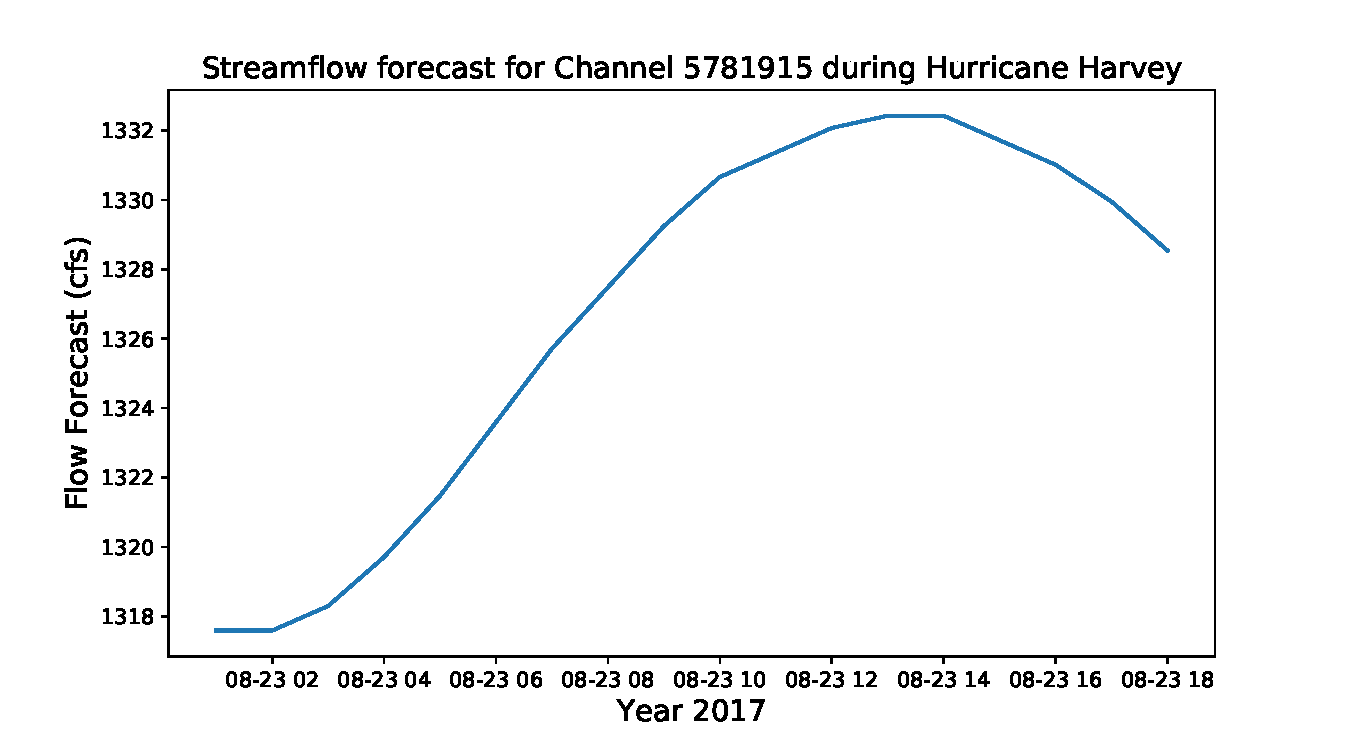
\includegraphics[scale=0.5]{Figures/nwm_hydrograph.pdf}
\caption{Time series plot for the accessed NWM streamflow dataset.}
\label{fig:data_component2}
\end{figure}


\subsection{Creating new models: Landlab}

Landlab is a Python-language library designed to support the creation, combination, and re-use of 2-D models \citep{hobley2017creative, barnhart2020short}. For the moment, let's presume that a model developer has identified input and output parameters, model state variables, and the governing equations and/or model rules. We might then synthesize the tasks of building the model (Section~\ref{sec:build}) into two types: (a) creating required data structures, and (b) implementing a numerical solution to the governing equations that act on those data structures. For example, most models need to represent the computational domain, including information  across the domain, and adjacency information describing how the different parts of the domain are connected to one another. This division is simplistic, and neglects many intricacies, yet it captures the fundamental activities of model building. 

\begin{figure}[h!]
\centering
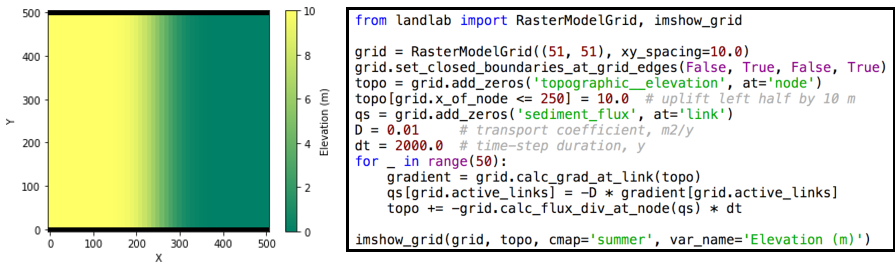
\includegraphics{Figures/simple_landlab_diffusion_model.pdf}
\caption{Example of a simple finite-volume numerical model of hillslope evolution, written in Python using the Landlab library. Model uses a diffusion equation to represent an evolving hillslope. The concise source code at right illustrates the use of a Landlab \textit{grid} object together with \textit{fields} and built-in functions for numerical gradient and divergence functions on these fields.}
\label{fig:landlabdiffusion}
\end{figure}


Landlab provides re-usable software infrastructure that addresses the most common needs for our two model-building tasks. For grid-based data structures, Landlab provides a \textit{grid} object to represent the computational domain and store \textit{fields} of state variables (Figure~\ref{fig:landlabdiffusion}). Landlab provides several two-dimensional grid types, which all share the same underlying graph-based data structures. Current grid types include regular raster, network, regular hexagon, and unstructured (Delaunay/Voronoi). For all grid types, the adjacency information and access to fields follows the same interface---making it easier for a model to work on multiple grid types.

\begin{figure}[h!]
\centering
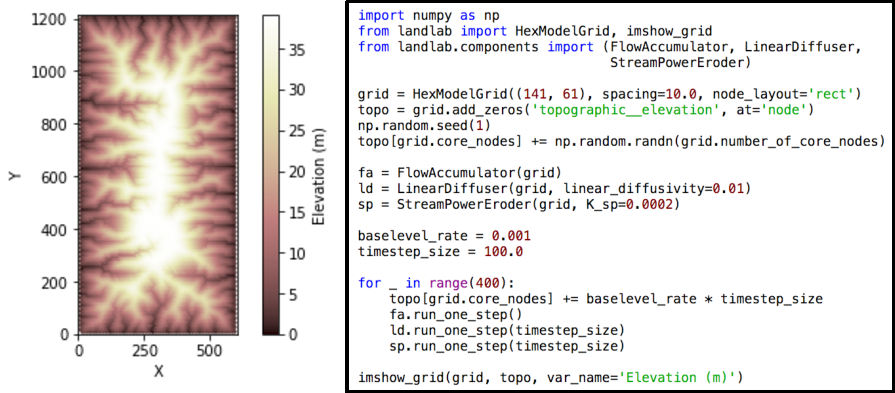
\includegraphics{Figures/landlab_component_lem.pdf}
\caption{Example of a simple landscape evolution model, written using the Landlab programming library. Model code at right illustrates the use of three \textit{components} to create the model.}
\label{fig:landlablem}
\end{figure}

To address the second model-building task, Landlab provides two capabilities. First is a set of numerical utilities that support common needs. These include, for example, the ability to calculate differences, gradients, fluxes, and divergences of values stored at fields. Second is a library of \textit{Components} (Figure~\ref{fig:landlablem}). Each Landlab component simulates a single process, such as routing of shallow water flow across a terrain surface \citep{adams2017landlab}, calculating groundwater flow \citep{litwin2020groundwaterdupuitpercolator}, modeling sediment movement in a river network \citep{pfeiffer2020networksedimenttransporter}, or simulating biological evolution across a landscape \citep{lyons2020speciesevolver}. Components are implemented as Python classes, and are derived from a common base class that defines common attributes, and enforces a minimum set of metadata for each component. If a researcher wishes to write the code for a numerical model, and the desired elements of that model have already been implemented as Landlab components, the model can be programmed efficiently by instantiating each component, and then executing the \texttt{run\_one\_step} method for each component within a loop (Figure~\ref{fig:landlablem}).

The \textit{Component} base class was designed to expose a Basic Model Interface (BMI; Section~\ref{sec:bmi}), which allows a Landlab component to be used as a BMI-enabled component.
Although we do not expect most Landlab users to directly use this alternate interface, the
component's BMI acts as a bridge that allows it to be incorporated into other BMI-friendly
frameworks and tools (e.g., pymt, \textit{dakotathon}).

The Python Modeling Toolkit (pymt; Section~\ref{sec:pymt})
is a model-coupling framework that provides tools for using and coupling BMI-enabled components,
written in a range on programming languages, which may not have been written with the intent
of operating within a coupling framework.
Operating as a BMI component, Landlab components act as isolated elements that no longer
share a common grid and data; when used in this mode, Landlab components require an input file that describes the grid, parameter values, and
initialization setup. This is by design and required by the BMI so that a user interacts
with the component as with any other BMI component without being aware of the inner workings
of a Landlab component.

% Through the such that conversion of Landlab Components to pymt components is trivial. 
% \todo[inline,color=yellow]{KRB: I think it would be best if Eric finished this section}

Despite the name, Landlab is not restricted to terrestrial processes. Its component collection includes, for example, components for coastal and marine processes such as tidal circulation and marine sedimentation. Its design is amenable to a wide variety of 2D grid-based numerical models and cellular automata applications. Landlab can be used, for example, to construct integrated source-to-sink models that treat the full geologic cycle, tracking sediment from its creation on land to its deposition in marine basins (Figure~\ref{fig:riftisland}).

\begin{figure}
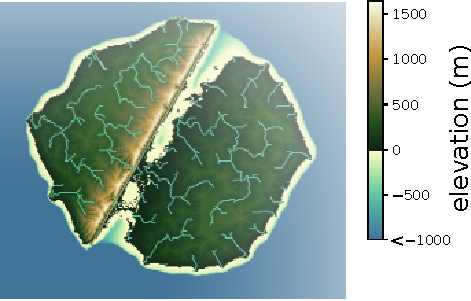
\includegraphics[width=10cm]{Figures/rift_island.pdf}
\caption{Snapshot from an integrated numerical model of landscape and sedimentary basin evolution. Domain size is 250 by 250 km. Simulation shows a hypothetical micro-continent with an active NNE-oriented extensional fault. Sea level varies stochastically; this particular snapshot captures a relative lowstand. Model was constructed using Landlab components for flow routing (\textit{FlowAccumulator, FlowDirectorSteepest, LakeMapperBarnes}), fluvial processes (\textit{ErosionDeposition}), marine sediment transport (\textit{SimpleSubmarineDiffuser}), and extensional faulting (\textit{KinematicExtender}). Colormap designed by \citet{thyng2016true}.}
\label{fig:riftisland}
\end{figure}


The design of Landlab supports a variety of usage styles. Interested users and/or developers may use Landlab to create models as Components, or as scripts that combine components. Alternatively, Landlab can be used to build stand-alone packages packages such as \texttt{terrainbento} \citep{barnhart2019terrainbento}, which combine Landlab components into a predefined set of models.

% GREGS NOTES:
% - relatively brief summary, pointing toward Hobley and Barnhart papers

% - include LL components as lighter-weight version of BMI components (because it's explicitly Python based, so don't need the extra overhead of BMI)

% - include mention of how a LL component gets converted to a pymt component

\subsubsection{HyLands: an example of a component-based integrated model}
  
The modular design of Landlab enables the development of numerical tools in an efficient manner. An example of a recently developed Landlab-built model is HyLands: a landscape evolution model that simulates mass wasting and sediment redistribution on hillslopes. The model was originally writte in a closed-source language \citep{campforts2020hylands}; translating the original code into Landlab converts the original product into a fully  open-source tool for the broader community, and provides a new process component to simulate landsliding. The grid engine and other tools available within the Landlab library enabled efficient implementation and provide capabilities for coupling with other, existing Landlab components. An example is the Stream Power with Alluvium Conservation and Entrainment (SPACE) component, which has been developed to simulate fluvial sediment transport and incision \citep{shobe2017space} and is showcased here as an example of model coupling with HyLands. 

The integration capabilities of Landlab, where new and existing components can be combined in a straightforward way, opens up new possibilities for applied environmental engineering and fundamental scientific research. For HyLands in particular, the coupling of a deep-seated landslide algorithm with a sediment routing system will (i) help on a more applied level to explore the impact of future changes in storm frequency on landslide occurrence and sediment dynamics \citep{Fan2019}, and (ii) on a more fundamental level to facilitate the investigation of the interaction between landslides and sediment dynamics over geological timescales. The latter is illustrated in Figure~\ref{fig:landslides}, where we use the Landlab software to simulate the impact of uplifting terrain on the formation of alluvial fans. Simulations are executed with and without landslide activity (Figure \ref{fig:landslides}a vs.\ Figure \ref{fig:landslides}b). Resulting magnitude-frequency and area-volume relationships for the simulated landslides are shown in Figure~\ref{fig:MF-landslides}. The evolution of the alluvial fans is further visualised in the movies listed in Table \ref{tab:LS-movies}. For details regarding the algorithms and physics supporting the HyLands component, see \cite{campforts2020hylands}.

\begin{figure*}
\includegraphics[width=14cm]{Figures/LS-Overview.png}
\caption{Illustration of HyLands model component. \textbf{a.}\ Time slices showing evolution of the landscape to steady state, without landsliding. The blue line represents the location of the river plotted in subplot (e). \textbf{b.}\ Same as (a), with landsliding. \textbf{c.}\ Sediment accumulation and the formation of alluvial fans. \textbf{d.}\ Landslide activity during the depicted time step. Red colors represent the logarithm of the landslide erosion, blue colors represent deposition. (e.) Shows the topographic and bedrock elevation (red and black line respectively) and the sediment thickness (orange line). The sediment flux is plotted against the right-hand y-axis (blue line). Note that, during landsliding, both pure landslide dams arise (red bumps on the profile) as well as irregularities in the bedrock profile (grey bumps). The latter originate from the river being redirected after landsliding, forming epigenetic gorges.}
\label{fig:landslides}
\end{figure*}

\begin{figure*}[t]
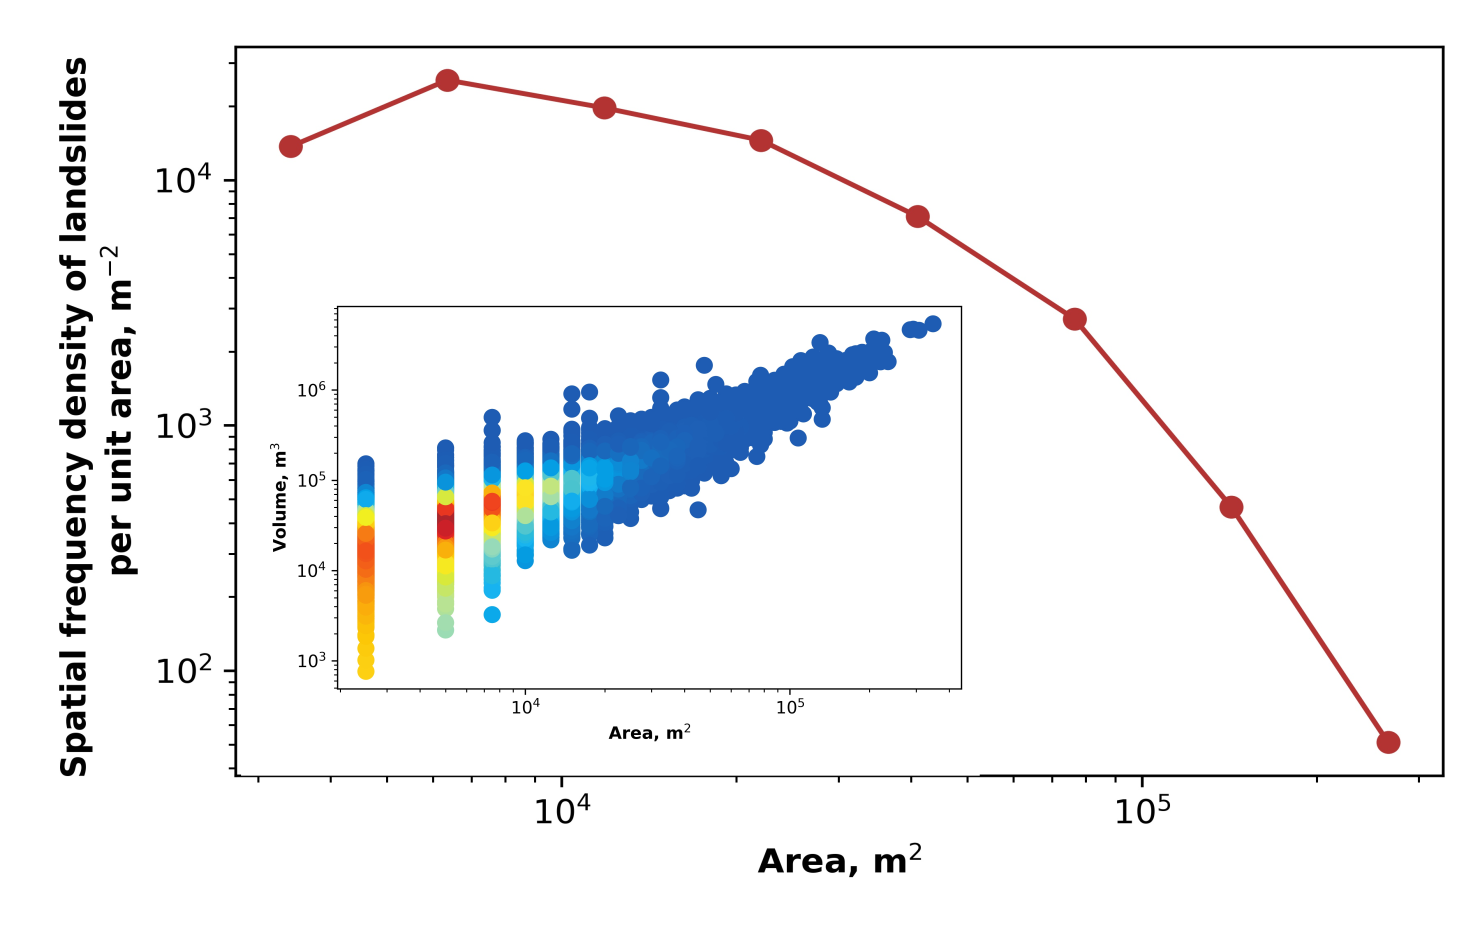
\includegraphics[width=10cm]{Figures/LS-Mag-Freq.png}
\caption{(\textbf{a}) Magnitude-frequency relationship of the landslides simulated with Landlab-HyLands (red dots) and illustrated in figure \ref{fig:landslides}. (\textbf{Inset}) Scatter density plot showing the simulated Area-Volume relationship.}
\label{fig:MF-landslides}
\end{figure*}

\begin{table}[htbp]
    %\Small
    \topcaption{Simulation movies created with Landlab-HyLands}
    \begin{tabular}{lll}
        \hline
        Scenario & Description & Link\\
        \hline\hline
        \verb|No landslides| &\verb|topography | & \url{https://youtu.be/c5d7T8eehxw} \\
        \verb|| &\verb|location of longest river|& \url{https://youtu.be/GqokukWi9cs} \\
        \verb|| &\verb|river profile |& \url{https://youtu.be/A_JZ9POfJ54} \\
        \verb|| &\verb|sediment thickness |& \url{https://youtu.be/t0_tel5fhbM} \\
        
        \verb|Landslides| &\verb|topography | & \url{https://youtu.be/1K_ceKYt9Nw} \\
        \verb|| &\verb|location of longest river|& \url{https://youtu.be/YkmbUTN7zlI} \\
        \verb|| &\verb|river profile |& \url{https://youtu.be/jyWgKTcMe74} \\
        \verb|| &\verb|sediment thickness |& \url{https://youtu.be/rwEBqGtHZs0} \\
        \verb|| &\verb|landslide erosion and deposition |& \url{https://youtu.be/_xoSm7p4ZxI} \\
    \hline
   \end{tabular}
   \label{tab:LS-movies}
\end{table} 

\subsection{Standard Names}

Ensuring interoperability when coupling models or selecting datasets as inputs to models requires accurate alignment of scientific variables. Scientific variables are complex concepts composed of multiple facets---a phenomenon or object of observation, the corresponding physical quantity being measured, spatiotemporal context for the phenomenon, spatiotemporal reference for the measured quantity, mathematical operations applied to transform the physical quantity, etc. Because of this, and because terminology varies across disciplines, the semantic mediation task---determining whether two variables represent compatible concepts---can be quite involved. In CSDMS, BMI works in tandem with the CSDMS Standard Names (CSN) \citep{peckham2013component} to ensure proper alignment between resources. The Standard Names were developed to standardize and unify the representation of scientific variables within CSDMS.

A CSDMS Standard Name contains two parts: an object part and a quantity part, with adjectives and modifiers (as prefixes) being used to help avoid ambiguity and identify a specific object and a specific, associated quantity. The quantity part may include one or more operation prefixes that create a new quantity from an existing quantity. An example related to surface-water hydrology is the runoff rate, for which the Standard Name is

\begin{verbatim}
land_surface_water__runoff_volume_flux
\end{verbatim}
The double-underscore separates the object (surface water on land) from the quantity (the volume flux of runoff). The word `flux' implies a quantity per time per surface area, and so the implied dimensions are length per time. 

As with all standard naming approaches, the Standard Names are limited in the amount of information they can represent because their data model and definitions are not explicitly represented. The Scientific Variables Ontology (SVO) \citep{stoica2018ontology, stoica2019scientific, stoica2019incorporating, stoica2020github, svoweb}, a blueprint for representing scientific variables utilizing a compact set of domain-independent categories, relationships, and modular design patterns, was developed to address these issues. In computer science, an \textit{ontology} is a system that attempts to capture and organize knowledge in a particular domain (in machine readable form), as understood by experts in that domain or subject area. In SVO, the CSN are represented with an explicit, formal model in machine-readable form using Semantic Web best practices \citep{berrueta2008best}. Because SVO is formalized, it can be used to enable searching, semi-automated generation of new variable representations, and inexact but sufficient variable alignments through logical reasoning.


%\subsection{OPTIONAL: Model analysis: Dakota and Dakotathon}

%- do we want to include this?
% NOTE THAT THERE IS AN EARLIER REFERENCE TO DAKOTHATHON
% I SUGGEST WE DO NOT WRITE ABOUT IT _THERE IS NOT MUCH USE OF IT

%\section{Software Development Practices}

%- VC

%- testing and CI

%- creating the documentation (and how much is enough?)
%   - API documentation vs examples (typically notebooks)

%- collaboration: issues and PRs


\section{Community Engagement}
\label{sec:community}

One of CSDMS' major activities has been the creation of a thriving community around Earth-surface dynamics modeling \citep{overeem2013strategies}. As of 2020, over 2,000 members, representing 552 institutions (144 US academic) and 71 countries, had joined the community.  CSDMS is, by design, a broad and deep coalition of members from disciplines reflected by five Working Groups and seven Focus Research Groups (Figure~\ref{fig:groups}).  From its inception, CSDMS has encouraged trans-disciplinarity by providing opportunities such as annual meetings, workshops, hackathons, and training events for domain scientists to interact with colleagues from other Earth and social science disciplines.  These connections are essential for knowledge exchange among community efforts and allow for wider penetration of new technology and ideas. Cross-pollination of ideas from these events and other community-member interactions have led to a variety of independently funded research projects. CSDMS has played a key role in shifting the paradigm to open code sharing in the Earth surface processes by facilitating resource sharing through model, data, and education repositories on the CSDMS web portal.  CSDMS also offers a variety of services to community processes and the geoscience subdiscipline of interest.   Along with their disciplinary expertise, researchers who work with computational models also need a strong foundation in programming, advanced computing, and data analytics  \citep{atkins2011national}.

Traditional Earth science education does not usually equip students with skills to use modern cyberinfrastructure and computing resources efficiently, or to become model developers \citep{campbell2013taking}. The Earth surface processes community critically needs a platform to teach modern programming practices and high-performance computing methods to develop innovative models that can be used to understand and predict how the Earth’s surface responds to environmental change and human influence.
The practice of modeling lies at the core of predictive Earth-surface sciences, and educators should engage students in building, testing, and applying models \citep{hestenes1996modeling,manduca2008making}, but we found from a review of course catalogs that in practice the undergraduate curricula of more traditional discipline-focused departments do not include this component \citep{campbell2013taking}. This issue is not entirely unique to Earth-surface sciences. The geosciences today are intensively quantitative, and there is an urgent need for a workforce with strong STEM skills \citep{national2012discipline}. The United States' National Science Foundation (NSF) recognizes as one of its `10 Big Ideas' that pathways are needed for educators to create a 21st-century workforce capable of effectively dealing with data \citep{king2017reimagining}. Moreover, an agile STEM workforce is considered a national priority \citep{atkins2011national}. Realizing this, CSDMS provides hands-on training opportunities during meetings. Some efforts are meant to build foundation---for example, via short courses that equip graduate students with skills in best programming practices. Other outreach efforts consist of short clinics, targeted to give potential users of cyberinfrastructure an active feel for certain models or computational techniques, or to provide an update to experts on new developments. More extensive separately organized hackathons bring together small science teams to work on solutions for more specific outstanding research problems.  In 2020, CSDMS inaugurated an immersive Earth Surface Processes Summer Institute for students and early career scientists, focused on capacity building for Earth-surface processes modeling.

\begin{figure}[h!]
\centering
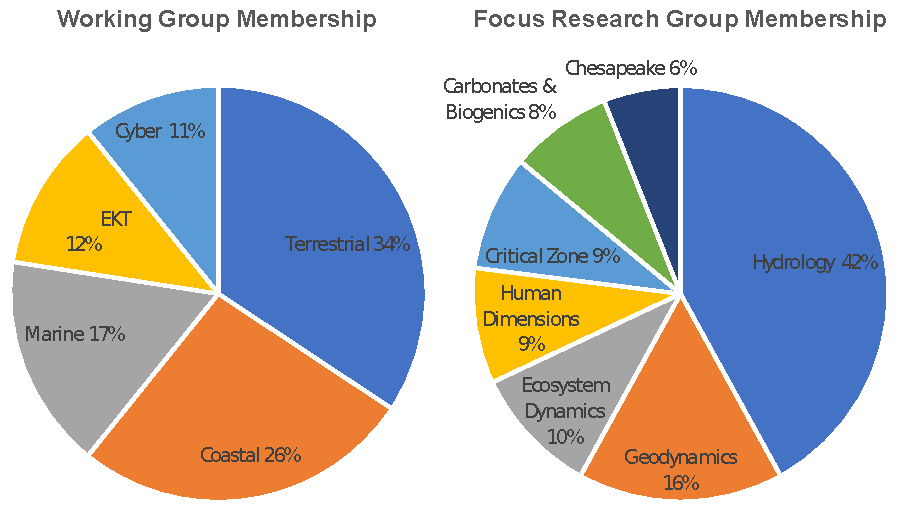
\includegraphics[scale=0.9]{Figures/working_and_focus_groups.pdf}
\caption{CSDMS Working Groups and Focus Research Groups.}
\label{fig:groups}
\end{figure}


\section{Discussion}
\label{sec:discussion}

In May 2020, the US National Science Foundation released a special report, prepared by the National Academy, on research opportunities in the Earth sciences \citep{nrc2020earth}. The report highlighted three unique types of research infrastructure: instrumentation, human infrastructure, and cyberinfrastructure. The report's recognition of cyberinfrastructure as a distinct form of research infrastructure is one indication of the critical role that computing now plays in the Earth and environmental sciences. Environmental modelling, and the software and culture-of-practice that support it, constitutes a key part of that cyberinfrastructure. Research software \textit{is} infrastructure, and deserving of the same care and attention as a laboratory or field station. So too are the professional research software engineers who devote their expertise to helping the community do computational work more efficiently, effectively, and sustainably.

The research enterprise benefits when modeling  software and tools are shared, coordinated, and interoperable, such that the six model operation tasks listed in Figure~\ref{fig:taxonomy} can be done efficiently and effectively. For the Earth surface sciences, the CSDMS Model Repository provides a community platform for finding and sharing model codes and related tools. In addition to acting as a valuable community resource, the Repository provides a solution to the growing mandate from journals and funding agencies to make research software openly available. The provision of standardized metadata and bibliographic information helps those who are looking for models to compare and evaluate the alternatives.

Simply providing source code and metadata is not enough, however. In order for Earth and environmental models to function as community resources, they must be usable, and one of the key dimensions of usability is interoperability. The BMI standard promotes interoperability by reducing the learning curve for executing and querying models, and by greatly simplifying the process of linking (one way) or coupling (two way) models. A model program equipped with a BMI becomes an interoperable, standardized component: an element of an integrated system, rather than an idiosyncratic stand-alone product. One of the key abilities offered by a BMI-enabled model is run-time control, query, and modification. Because BMI supports step-wise execution, a user can effectively pause a model in mid-run to inspect its state variables, and modify parameters or data. This capability allows iterative, loop-based coupling of models using simple scripts. The ability to query and modify values also enables tighter coupling. For example, if  component models are treated as representing individual terms in a governing equation, a coupling script can use BMI functions to query each component's derivatives, construct a matrix, solve it, and then pass the updated state variables back to the individual components.

One advantage of BMI is that it is language agnostic, and can in principle be implemented in nearly any programming language. It can, for example, accommodate legacy codes written in Fortran. The disadvantage of language flexibility is that BMI addresses the least common denominator, and therefore does not take advantage of the more advanced features available in some languages, such as object-oriented capabilities. To some extent this disadvantage can be addressed by building more specialized, language-specific interfaces in parallel with a BMI. For example, Landlab components, which are implemented as classes, use a lightweight, Python-specific interface that takes advantage of that language's object-oriented capabilities, advanced data types, and parameter-passing syntax. At the same time, Landlab also includes functionality to translate any of its components into a standard BMI component, so they can be integrated with components written in other languages.

The flexibility that BMI offers has led to its adoption in a variety of different applications, including US Geological Survey rainfall-runoff models \citep{markstrom2015prms,regan2018description,regan2019us}, hydrodynamic modeling \citep[including flagship models developed by Deltares and the Netherlands eScience Center,][]{hoch2019advancing,hoch2019evaluating}, delta and coastline evolution modeling \citep{ratliff2018exploring}, and modeling of methane emissions \citep{fox2020agent}, to name a few. One disadvantage of a standard interface like BMI is the extra up-front investment in program development. Researchers may not perceive value in adding a standard interface to a legacy code, or writing it into a new code. However for codes whose scope merits repeated re-use, this effort usually more than pays for itself. Code written to a standard like BMI tends to be more modular and therefore easier to maintain. Existing templates for common languages in the Earth and environmental sciences make the process of providing a BMI to a new program is relatively painless: just a matter of filling in a set of pre-defined function names and signatures \citep{hutton2020basic}. Adding a BMI to an existing legacy model can be a bit more involved, depending on how the program code is structured, because it often requires some degree of refactoring. Even in that case, we find that adding a BMI to a legacy model often makes that code more understandable and adaptable.

The variety of different programming languages used in the Earth and environmental sciences community presents a barrier to interoperability. The majority of models and tools in the CSDMS Repository are written in C, C++, Fortran, Python, and Matlab (Figure~\ref{fig:languages}). Other languages used in CSDMS constituent communities include R (especially in ecosystem dynamics) and NetLogo's java-based scripting language (for agent-based modeling). Julia, a relatively new high-level language oriented toward numerical computing, also seems to be growing in popularity in the science community. Crossing the language barrier requires language-bridging tools. Translating the existing wealth of legacy code into a single, common language would be impractical, even if the community could agree on which language to use. A more effective solution is to \textit{librarize} models and tools \citep{brown2014run} as components that can be accessed and executing through a high-level scripting language. In CSDMS' case, the Babelizer tool provides this capability for codes written in C, C++, and Fortran, using Python as the bridging language.

Librarization can be applied to data sets too. The CSDMS Workbench accomplishes this with Data Components that provide function-call access to various data sets. Using the BMI syntax for data access removes the need to worry about data formats, and makes it easier to swap between data sets and models (for example, data versus model of ocean-wave properties) as components in a linked system. In this case, the BMI does not replace the more sophisticated data-access capabilities of a language-specific library like xarray, but it has the advantage of providing a consistent interface across multiple languages.

For building and modifying numerical models, the CSDMS Workbench provides Landlab as a Python-specific solution for 2D, grid-based applications. Experience with Landlab since its introduction has shown that a library of model `building blocks' can greatly reduce barriers on the software side of model creation. One indicator of the success of this approach is the growing number of  Landlab-built models created by doctoral students as part of a larger body of dissertation research \citep[e.g.,][]{adams2017landlab,gray2017off,shobe2017space,lai2018modeled,langston2018developing,schmid2018effect,strauch2018hydroclimatological,glade2019canyon,reitman2019offset,carriere2020impact,litwin2020groundwaterdupuitpercolator}. The ability to assemble models out of reusable `process components' allows for rapid construction of complete, multi-element models. One example of the value of rapid model assembly is a recent  comparative testing and calibration study of long-term landform evolution models \citep{barnhart2020inverting1,barnhart2020inverting2}. The study authors used Landlab to develop a Python package for multi-model analysis of drainage basin evolution \citep{barnhart2019terrainbento}. The package allowed for the exploration and testing of more than 30 mathematically distinct models, as alternative hypotheses---a feat that would not have been possible with a traditional monolithic modeling code. This example illustrates how flexible, component-based modeling software promotes hypothesis testing. 

Experience with BMI, pymt, and Landlab highlights the critical importance of documentation, consistent with the findings of \citet{lawrence2015science}. Tutorial examples in particular provide a starting point that users can build on. Embedding tutorials in Jupyter Notebooks provides an effective way to combine descriptive text, program code, plots, and formatted mathematics. For reference-level documentation, document generator tools like Sphinx and doxygen translate internal documentation (comment blocks inside source code) into nicely formatted, web-accessible reference material.

A successful community cyberinfrastructure for numerical modeling requires more than just technology. It also takes community building and coordination. In the case of CSDMS, the community centers around common interest in a broader theme (Earth-surface processes) and a common approach (modeling). Activities such as meetings, workshops, hackathons, and webinars can help draw attention to new tools and methods, provide education in their use, and contribute to building a culture of resource sharing.

One of the biggest challenges to a fully functional community software ecosystem in Earth and environmental modeling is a lack of formal training in computational skills. Most geoscientists are self-taught programmers, and generally unaware of practices and tools that would make their work more efficient and sustainable. CSDMS and other community facilities have had some success in addressing this need with workshops, webinars, and summer schools, but there remains a need to scale up these efforts. Geoscience researchers should not need the equivalent of a computer science degree to perform computational research, but in our experience there is a basic set of skills that can make a big difference, yet which relatively few geoscientists possess. Potential solutions range from regular university-based, geoscience-oriented courses, to focused, community-led summer courses (like CSDMS' ESPIN, or the IsoCamp program for isotope geochemistry), to fully online courses. Questions of credit and funding inevitably arise, as does the issue of how to squeeze more material into already-packed curricula.  

Another challenge revolves around incentives. The community as a whole clearly benefits from a FAIR and sustainable research software ecosystem. As noted above, the advent of software journals and peer-reviewed repositories (such as COMSESnet and pyopensci) provides one mechanism to encourage the creation of lasting digital products. The reproducibility movement provides another useful push, and has led journals and funding agencies to raise their standards for sharing and accessibility of software and other digital products. To take advantage of this momentum, hiring and promotion committees at universities and research organizations need to acknowledge the value of contributions to high-quality research software. Professional societies can contribute by offering awards that recognize contributions to cyberinfrastructure.

The third major challenge is support. Our experience with CSDMS demonstrates that a modest investment in community-oriented computing can have a substantial positive impact on research productivity. By investing in stable community repositories, interoperability standards, and software libraries and frameworks, a funding agency can increase the impact of its portfolio by incentivizing a shared, reusable and ever-improving community infrastructure of models, tools, and expertise. A key to making this approach scalable, in addition to incentives, is to provide sufficient documentation and consulting support to enable community members to create research cybertools that are Findable, Accessible, Interoperable, and Reusable. We have found from our own experience that consulting support is an especially important piece. Projects that include a professional research software engineer in their team---even if it is just at the level of general design advice, informal education, or help overcoming technical obstacles---tend to be much more likely to produce robust, flexible, sustainable software as a lasting broader impact of a project.

Computational modeling in the Earth and environmental sciences has come a long way since the dawn of the 3rd millennium. The possibilities of a coordinated, community-wide cyber-ecosystem are starting to emerge. Fully achieving this vision will require a combination of education, incentives, and support. Universities, research agencies, and individual researchers all have a role to play.


\section{Acknowledgements}

The Community Surface Dynamics Modeling System (CSDMS) is supported by the US National Science Foundation (NSF) (1831623). Initial development of Landlab was supported by the NSF SI2 program (1450409). The Permafrost Toolbox was supported by NSF OPP (1503559 to IO and MP). ESPIN is supported by NSF-CISE (1924259 to IO, MP and BC). Additional sources of support include EarthCube (2026951 to GT and EH), and an NSF postdoctoral fellowship (1725774 to KRB). %, and  ...[ADDITIONAL SOURCES HERE]


\bibliography{gt_library}
\bibliographystyle{agu08}

\end{document}
